\documentclass[12pt,a4paper,english]{book}

\usepackage[T1]{fontenc}
\usepackage[utf8]{inputenc}
\usepackage[english]{babel}
\usepackage{amsmath}
\usepackage{amsfonts}
\usepackage{mathtools}
\usepackage{fancyhdr}
\usepackage{graphicx}
\usepackage{hyperref}
\usepackage{tikz}
\usepackage{listings}
\usepackage{float}
\usepackage{csvsimple}
\usepackage{pgfplots}
\usepackage{subcaption}
\usepackage[titletoc]{appendix}
\usepackage{rotating}
\usepackage{textcomp}

\usepackage{sty/pgf-umlsd}

\usetikzlibrary{arrows,calc,shapes,positioning,chains,fit,decorations.pathreplacing}

% Header and Footer Style
\fancyhead{}
\fancyhead[R]{\slshape Patrick Steinhardt}
\fancyhead[L]{\slshape\nouppercase{\rightmark}}
\fancyfoot{}
\fancyfoot[C]{\thepage}
\renewcommand{\headrulewidth}{0pt}
\renewcommand{\chaptermark}[1]{\markright{\thesection\ #1}}

% No identation
\setlength\headheight{15pt}
\setlength\parindent{0pt}

\bibliographystyle{alpha}

\widowpenalty10000
\clubpenalty10000

\lstset{language=C}
\lstset{captionpos=b}

\pgfplotsset{
    discard if/.style 2 args={
        x filter/.append code={
            \edef\tempa{\thisrow{#1}}
            \edef\tempb{#2}
            \ifx\tempa\tempb
                \def\pgfmathresult{inf}
            \fi
        }
    },
    discard if not/.style 2 args={
        x filter/.append code={
            \edef\tempa{\thisrow{#1}}
            \edef\tempb{#2}
            \ifx\tempa\tempb
            \else
                \def\pgfmathresult{inf}
            \fi
        }
    }
}

\pgfplotscreateplotcyclelist{custom}{
    dotted, red, every mark/.append style={solid, fill=red}, mark=otimes*\\%
    dashed, blue, every mark/.append style={solid, fill=blue}, mark=square*\\%
    densely dotted, orange, every mark/.append style={solid, fill=orange},mark=triangle*\\%
}

\pgfplotsset{
    cycle list name=custom
}

% Titel and author
\title{A Protocol for Connecting Distributed Resources}
\author{Patrick Steinhardt}
\date{Berlin, July 26, 2016}

\begin{document}
    \pagestyle{plain}
    \pagenumbering{gobble}
    \begin{titlepage}
    \makeatletter
    \begin{center}
        \vspace*{2cm}
        {\Large Freie Universität Berlin}\\
        {\large Department of Mathematics and Computer Science}
        \vspace*{3.5cm}

        {\Large \@title}\\
        \vspace*{0.5cm}
        {\large \@author}

        \vspace*{3cm}

        \textbf{Master's Thesis}\\
        in partial fulfillment of the requirements for the degree of\\
        Master of Science\\
        \vspace*{1cm}
        \@date

        \vspace*{\fill}

        \begin{tabular}{r|l}
            \bf \llap{First reviewer} & \bf \rlap{Second reviewer} \\
            \llap{Prof. Dr.-Ing. Volker Roth} & \rlap{Dr.-Ing. Achim Liers}
        \end{tabular}
    \end{center}

    \makeatother
\end{titlepage}

% vim: ft=tex tw=0

    \vspace*{\fill}


\begin{minipage}{0.7\textwidth}
    This work is licensed under the Creative Commons Attribution-ShareAlike 4.0 International License.
    To view a copy of this license, visit \url{http://creativecommons.org/licenses/by-sa/4.0/}.
\end{minipage}
\hfill
\begin{minipage}{0.25\textwidth}
    \includegraphics[width=\textwidth]{resources/by-sa.eps}
\end{minipage}

\pagebreak

% vim: tw=0

    \subsection*{Affirmation}

I hereby declare to have written this thesis on my own.
I have used no other literature and resources than the ones referenced.
All text passages that are literal or logical copies from other publications have been marked accordingly.
All figures and pictures have been created by me or their sources are referenced accordingly.
This thesis has not been submitted in the same or a similar version to any other examination board.

\vspace{4em}

\begin{tabular}{c}
    \rule{7cm}{1pt}\\
    \makeatletter\@date\makeatother
\end{tabular}

% vim: ft=sh tw=0


    \tableofcontents
    \listoffigures

    \cleardoublepage

    \pagestyle{fancy}
    \pagenumbering{arabic}
    \setcounter{page}{1}

    \chapter{Introduction}

\begin{quote}
    The most profound technologies are those that disappear.
    They weave themselves into the fabric of everyday life until they are indistinguishable from it. \cite{weiser1991computer}
\end{quote}

The above quote is how Mark Weiser introduces his paper on how he imagines the computer of the 21st century.
The computer is about to disappear, become our go-to technology for many different things without even noticing that we are actually using a computer.
Nowadays many see this paper as a vision for how computing should work: integrate all everyday-objects like fridges, watches or even light bulbs with computers and orchestrate them all together using a simple interface.
This is how the Internet of Things is envisioned.

But are we even close to this vision?
Every month, there are new devices announced which are able to communicate via the internet and be remote-controlled by people.
But with most devices, there is a recurring theme: these devices are insecure, use no real authentication or even encryption.

But we do not even have to look as far as ``Internet of Things''-enabled devices.
In his seminal paper, Mark Weiser goes on to talk about how devices seamlessly integrate with each other.
But as of today, we are not even able to easily handle interconnectivity for the most basic of tasks: just try to transfer a simple file from a computer with one operating system to another computer with a different operating systems or display a graphical application on the screen of a colleague.
So when even those simple tasks are not trivial to do, one can argue that we are far away from the Internet of Things as imagined by Mark Weiser.

In this thesis, our aim is to develop a protocol which enables more seamless integration between devices.
Given a set of devices, each of them shall be able to host a set of services, where every service provides certain functionality.
Other devices shall be able to bind to these services and use their provided functionality.
But most importantly, we want the binding process to be as hassle-free as possible for the user.

Given that smart phones are as ubiquitous as they are today, they become a natural match in guiding this process:
a user should be able to simply connect his home server with the display at work by pressing a button on his smart phone, where the complete setup following the button press is done by the service framework.

One of the most important aspects is to have the framework do its work in a way such that every action is fully authenticated and encrypted.
No entity shall be able to talk to any service for which it has no access rights and no adversary shall be able to gain knowledge about what an entity and the services its connect to are transmitting.

In order to fulfill these requirements, we develop a protocol based on public keys and capabilities.
The permission to interact with a service is granted when an entity with a certain public key possesses the capability to access that service.

\bigskip

The thesis proceeds as follows:
In the second chapter, we will detail the problem that this thesis is about to solve.
The third chapter will describe the architecture of the developed protocol in a theoretical manner.
The fourth chapter presents the implementation details of the architecture, followed by a chapter in which we present benchmarking results for this implementation.
The sixth chapter will discuss the ability of protocol and implementation to solve the actual problem.
Finally, we will summarize our findings.

% vim: ft=tex tw=0

    \section{Problem definition}

In this chapter, we will define the actual problem and outline which parts of the overall problem we do not want to solve.
We will further state our assumptions regarding the security model and abilities of the adversary.

This thesis tries to solve the problem of connecting different resources provided by servers with each other using a single protocol.
The protocol shall be able to discriminate these resources, be able to configure them when trying to connect with its provider in order to use the resource and then subsequently use the actual resource in a way it is intended to be used.
Furthermore, it should be possible to steer the complete protocol by use of a third devicee, the controller, which shall able to connect an agent with a service provider without requiring physical access to either of both parties.

The actual architecture should be service-agnostic, that is we do not try to solve the problem of underlying communication protocols used when a service has been started by an agent.
As such, we want to be indifferent to the actual service protocol that is used, given that the protocol is actually able to talk via the network protocol TCP/IP.
While some protocols will need to be developed which are specific to this service infrastructure and where their protocol is actually be defined by us, these are only special cases.

As the thesis' title states, we want to solve the problem of connecting \emph{distributed} resources.
So in fact, we do not want to rely on centrally available computing infrastructure, but instead users should be able to discover services without previous knowledge of the network environment and without having to provide any kind of central servers.
To achieve the requirement, we also develop a service discovery protocol which can be used to locate services without any third party.
Nevertheless, the service discovery part is not a focus of this thesis as a multitude of different services exist which already handle service discovery.

A central point to this thesis is to implement the protocol in a secure way.
We explicitly exclude the implemented service discovery protocol from this requirement, as its purpose is to discover previously unknown services where it is impossible to authenticate the service without any prior knowledge.
Barring this initial step, all communication between services and their peers shall be fully authenticated and encrypted such that no adversary is able to recover messages exchanged between these parties.

To achieve this goal, the first assumption made is that peers have previously exchanged long-term public signature keys with each other through some kind of side-channel.
The problem of key exchange is not solved in this thesis.

We further assume that the adversary has the ability to interpose all communication paths.
He is able to read all traffic between peers, modify or replay messages sent or inject arbitrary messages.
On the network layer, the adversary is able pretend to be either of these peers.
So in the end, the adversary has complete control over all network functionality and is able to spoof identities of all participating peers.

The adversary has no access to key material, though.
That is, he cannot in any way encrypt, decrypt or sign any messages in the name of any peer without previously gaining access to the key material in any way.
Furthermore, we assume that operators of provided services are honest and did not permit access to the service's long-term signature key pair to the adversary.

The last assumption is that all services and peers have a secure computing environment which is not compromised by the adversary.

% vim: ft=tex tw=0

    \section{Architecture}

We will now take a look at the high-level architecture of the whole application stack.
That is we will cover the initial process of a client dicsovering available servers in a local network, querying found servers and then connecting to a specific service.
Let us first define the terms.

\begin{description}
    \item[Server]\hfill\\
        A server is a single entity which may host several services.
        As such, he has an identity which is represented to clients and connecting services via a public signature key.
        The server is responsible for handling the process of service discovery.
    \item[Service]\hfill\\
        A service is hosted on the server which announced the service's availability.
        Services provide a certain bit of functionality, e.g. they may provide a display for use by other parties or provide the functionality of executing a certain program.
    \item[Session]\hfill\\
        When a client wants to start a certain service, he will first have to initiate a session which can then be used to actually start the service.
        Upon sending an identity and a set of parameters to the service, it will create a new session and return an identifier for the session.
        The session identity is then able to connect to the service using the identifier and as such start using its functionality.
    \item[Client]\hfill\\
        Clients are parties which have the intent to invoke a certain service.
        A client has an identity, as well, which is used by services to identify their permissions and to establish sessions.
\end{description}

We will now take a look at the actual process how a single client will proceed if it wants to invoke a certain set of services (see figure \ref{fig:overview}).

\begin{figure}[H]
    \centering

    \begin{tikzpicture}[
            connection/.style={draw, -triangle 45},
            server/.style={draw, rectangle, minimum height=1cm, minimum width=0.4cm},
            service/.style={draw, ellipse}
        ]

        \node (client) {Client};

        \node[server, left=3.0cm of client,  yshift=0.8cm] (s1) {};
        \node[service, left=of s1] (display) {Display};
        \path[draw] (display) -- (s1);

        \node[server, above=3.0cm of client, xshift=2.0cm] (s2) {};
        \node[service, above=of s2, xshift=-1.5cm] (cpu2) {CPU};
        \path[draw] (cpu2) -- (s2);
        \node[service, above=of s2, xshift=+1.5cm] (display2) {Display};
        \path[draw] (display2) -- (s2);

        \node[server, below=3.0cm of client, xshift=3.0cm] (s3) {};
        \node[service, right=of s3] (invoke) {Invoke};
        \path[draw] (invoke) -- (s3);

        \path[connection, bend right=20] (client) to node[above] {1.} (s1);
        \path[connection, bend right=20] (client) to node[left] {1.} (s2);
        \path[connection, bend right=20] (client) to node[below left] {1.} (s3);

        \path[connection, bend left=20, transform canvas={yshift=-1mm}] (s1) to (client);
        \path[connection, bend left=20, transform canvas={xshift=+1mm}] (s2) to (client);
        \path[connection, bend left=20, transform canvas={yshift=+0.5mm, xshift=+0.5mm}] (s3) to (client);

        \path[connection, bend left=20] (client) to node[below] {2.} (s1);
        \path[connection, bend right=20, transform canvas={yshift=+1mm}] (s1) to (client);

        \path[connection, bend left=20] (client) to node[above right] {3.} (s3);
        \path[connection, bend right=20, transform canvas={yshift=-0.5mm, xshift=-0.5mm}] (s3) to (client);

        \path[connection] (client) to node[right] {4.} (s3);
        \path[connection, bend left=30] (s3) to node[below] {5.} (s1);
    \end{tikzpicture}

    \caption{Overview}
    \label{fig:overview}
\end{figure}

Let us assume that Alice wants to connect a display provided by one service with an executable that she has running on her own server.
Both servers are part of the same network and can thus connect to each other without problems.

The initial step is to discover the devices taking part in the protocol.
After connecting to the internal network with her mobile phone, Alice will start the client application and initiate the service discovery.
The service discovery will broadcast a message into the network and alert the servers that a new client has appeared which wants to discover all servers with their services.
Alice will now receive announcements of the three available servers in the local network together with their identity and a list of services they host.
One of these servers is her own computer running the executable she wants to connect to the display, which is already marked in her application as being known and verified.

Alice compares the remaining server's identities to the one Bob gave her to find the server sharing the display.
As she trusts Bob, she also trusts that the identity given to her is actually valid and that the attached server is of benign nature.
She now spotted the server on the list and recognizes that it indeed exposes a display service, which she now queries for further details.
The server announces that the service is actually backed by the xpra service, which is a specific implementation used for graphics forwarding.
As Alice is already running her local application inside an xpra instance, everything is fine and she proceeds.

Now comes the time of actually connecting to the service.
Alice establishes a connection to the newly discovered display service and creates a new session.
As she does not want to connect herself but instead wants her server to connect to the display, she specifies her server's identity as the session owner.
The server creates the new session and tells Alice its identifier.

As the session is established and ready for use, Alice now creates a new session on her own server, this time setting her own identity as the session owner.
Along with the identity, she also sends over details about the other service as well as the session identifier she just obtained as parameters which should be used by her own service.
She now invokes her own service, which goes on to start the session with the display service stored in the session's parameters.
The locally running application is now forwarded to the display until the session is terminated.\\

Summarizing the above, the following steps are required to connect to a service:
\begin{enumerate}
    \item Discover services in the local subnet by broadcasting messages
    \item Query a specific service on a server for its details
    \item Establish a session with a set of parameters and specify a session owner
    \item Let the owner connect to and thus start the session
\end{enumerate}

We will discuss how these steps are implemented in section \ref{sec:protocol}.
But first, let us examine how data is transmitted on the wire.

\subsection{Low-level protocol}
\label{sec:low-level-protocol}

The low-level protocol determines how the actual packets sent between client and server are constructed.
It specifies a common format independent of the actual transport layer that is used to guarantee a common understanding of how to handle incoming bytes.
The protocol is currently designed to be used over either TCP or UDP but should be generic enough to be used for other transport layers.
We will concentrate on describing design choices based on TCP and UDP transport layouts only, though.

\subsubsection{Package boundaries}

In contrast to TCP, UDP is a connection-less protocol that is based upon packages instead of a data stream.
As clients have to distinguish these packages in the UDP protocol, they have their package length attached to the package header.
As such it is guaranteed that when receiving a single package over UDP we know package boundaries and thus can split incoming packages by these boundaries.
On TCP we have to develop our own solution to distinguish single packets, so we need to design a package format which is able to specify package boundaries.

The initial design simply prefixed every single package with an unencrypted package length fixed to four bytes in network byte order.
This allows the client to initially receive four bytes, convert these to host byte order and subsequently receive the amount of bytes specified.
While easy to implement this has several disadvantages.

The most obvious disadvantage is that the package length was always transmitted unencrypted and without any message authentication code.
This allows potential adversaries to do easily traffic analysis based on package lengths or drive an attack by simply tampering with the length.
As the receiver of the package cannot verify the package's length in any way he has to trust it and thus may receive invalid packages.

In order to solve the problem the most obvious solution would be to simply encrypt the length and attach a message authentication code.
By doing so we would prevent the adversary of knowing the following data's length and prevent that he is able to tamper with it.
Like this, we obviously gain a boost in security compared to sending package length's in plain text.

On the other hand, the adversary is still able to observe actual package lengths.
In the case of UDP being used as a transport layer this is trivial:
An adversary can simply inspect package headers and thus extract the actual package length, as data is in the general case sent in a single package.
In the case of TCP where no actual package length is encoded in the TCP header this is a little bit more involved but in many cases still feasible as client and server are likely to exchange single messages by turn.
So by substracting the prefixed package length and its message authentication code from the total bytes sent in one turn we are able to gain knowledge of the actual message length with a high probability.

Due to this we are effectively giving the adversary an decryption oracle as he is able to correlate package lengths and their encrypted representations.
Furthermore it becomes much easier for an adversary to analyze traffic by inspecting actual package lengths.
\\\\

To fix the problem we send blocks of a fixed length instead of prefixing every package with an encrypted length.
The initial fixed-length block is prefixed with the overall length of the assembled package.
If the overall length exceeds the length of the remaining bytes of the first fixed length block, then the complete block is assembled by concatenating the first block excluding its length prefix and all subsequent blocks until the announced length is received.
The last block is right-padded with zeroes until its length matches the block length.
The package length is only encoded in the first block.

The following example demonstrates the package format for unencrypted packages.
We assume a fixed length block size of 64 bytes.
If a party now wishes to transfer a package of 80 bytes the package will get split into two blocks.
The first block is prefixed with four bytes containing the actual package length and filled with the initial $64 - 4 = 60$ bytes.
The second package is filled with the remaining $80 - 60 = 20$ bytes and right-padded with $64 - 20 = 44$ zeroes.
Figure \ref{fig:unencrypted-package-format} visualizes the block's contents.

\begin{figure}
    \center

    \begin{tikzpicture}[
            every node/.style={ minimum width=6mm, minimum height=8mm },
            start chain=1 going right,
            start chain=2 going right,
            node distance=-0.15mm
        ]

        \node[draw, on chain=1, minimum width=8mm] {len};
        \node[draw, on chain=1, minimum width=88mm] {60 bytes of data};
        \node[left=1cm of 1-1] {Package 1};

        \node[draw, on chain=2, minimum width=40mm, below=1cm of 1-1.west, anchor = west] {20 bytes of data};
        \node[draw, on chain=2, minimum width=56mm] {padding};
        \node[left=1cm of 2-1] {Package 2};
    \end{tikzpicture}

    \caption{Unencrypted package format}
    \label{fig:unencrypted-package-format}
\end{figure}

The second example (see figure \ref{fig:encrypted-package-format}) demonstrates the package format for an encrypted connection.
In contrast to unencrypted packages there is an additional message authentication code attached to each split package which is now assumed to be 16 bytes long.

\begin{figure}
    \center

    \begin{tikzpicture}[
            every node/.style={ minimum width=6mm, minimum height=8mm },
            start chain=1 going right,
            start chain=2 going right,
            node distance=-0.15mm
        ]

        \node[draw, on chain=1, minimum width=24mm] {MAC};
        \node[draw, on chain=1, minimum width=8mm ] {len};
        \node[draw, on chain=1, minimum width=64mm] {44 bytes data};
        \node[left=1cm of 1-1] {Package 1};

        \node[draw, on chain=2, minimum width=24mm, below=1cm of 1-1.west, anchor = west] {MAC};
        \node[draw, on chain=2, minimum width=54mm] {36 bytes data};
        \node[draw, on chain=2, minimum width=18mm] {padding};
        \node[left=1cm of 2-1] {Package 2};

        \draw [decorate,decoration={brace,amplitude=10pt}] (1-2.north west) -- (1-3.north east) node[midway,yshift=7mm] {encrypted};
        \draw [decorate,decoration={brace,amplitude=10pt,mirror}] (2-2.south west) -- (2-3.south east) node[midway,yshift=-7mm] {encrypted};
    \end{tikzpicture}

    \caption{Encrypted package format}
    \label{fig:encrypted-package-format}
\end{figure}

The client will now fetch the initial fixed-size block
If the connection is encrypted, he will decrypt it and verify its message authentication code.
Now we inspect the first four bytes to gain knowledge about the total package length -- if it exceeds the amount of bytes sent in the initial message, we will receive, decrypt and verify all following packages until all bytes are received.
Finally, we concatenate the blocks to obtain the complete package.

\subsubsection{Cryptography}

All connections except the initial service discovery are authenitcated and encrypted to keep information safe.
Encryption is done via secret-key authenticated encryption with an encryption key shared between both parties.
The key is an ephemeral key generated in an authenticated way via Diffie-Hellman key exchange when establishing the connection (see section \ref{sec:connection-establishment} for more details on the actual key exchange).

As the generated key is an ephemeral key which is not to be re-used in later sessions we are able to use a simple counter mode for nonces.
That is, on initial connection the client per definition has a nonce of value $0$ and the server has a nonce of value $1$.
Whenever either the client or server encrypts and sends a new block, its nonce is incremented by $2$.
On the receiving side we increment the remote nonce by $2$ every time we receive an encrypted block.
This guarantees (given nonces of sufficient length) that nonces are never repeated as collisions between client and server nonce are impossible and nonces are monotonously increasing.

The algorithm used for encryption is the Salsa20 stream cipher by Daniel J. Bernstein \cite{bernstein2008salsa}.
It is a family of 256-bit stream ciphers to designed to be used in a wide range of cryptographic applications.
It uses a 256-bit key and a 64-bit nonce and expands them into a $2^{70}$-byte stream.
Encryption for a plain text message with $n$ bytes is done by xor'ing the plaintext with the first $n$ bytes of the stream.
Decryption is done likewise, xor'ing the ciphertext with the first $n$ bytes of the same stream.
We specifically use the Salsa20/20 stream cipher, which is a 20-round stream cipher, compared to reduced-round ciphers specified by Daniel J. Bernstein.

The algorithm used for message authentication is the Poly1305 message authentication code by Daniel J. Bernstein \cite{bernstein2005poly1305}.
Poly1305 takes a 32-byte key and a message and produces a 16-byte tag that authenticates the message.
The key for the combination of Salsa20/Poly1305 is generated by deriving a subkey from a tuple of key and nonce used for encrypting the actual message.

\subsubsection{Message exchange}

Exchanging data between hosts poses several questions.
Consider we want to send a data structure over to another host.
The naive approach would be to simply stream over the in-memory representation of the structure and let the receiver interpret the data stream as the corresponding structure.
This naive approach is not even guaranteed to work for two hosts running on the same architecture, as for example the compiler may choose to re-arrange structure entries.
The approach finally falls flat when considering different operating systems with different application binary interfaces or even different memory layouts, e.g. different byte orders.

The problem of correctly serializing data is not trivial and thus we choose to not handle the problem ourselves but let a library designed for this problem handle serialization.
Google Protocol Buffers \cite{varda2008protocol} implement a method for serializing structured data in platform- and language-independent way.
Protocol Buffers come with a way to specify interface descriptions that describe how data is structured in a certain message type.
These interface descriptions are then compiled to language-specific code that can be imported via language-specific constructs.

One inherent benefit of this approach is that we are able to re-use the interface definitions across multiple sites.
In particular, we use the same interface definitions across the command line client and server which are both written in C, and the Android controller which is written in Java.

The whole protocol is built upon these interface descriptions with the only exception being when we forward application-specific data between two specific services.
As we do not want to know about the specific protocols they use in order to be generic as possible we simply relay data from and to both service end points.
Otherwise all message exchanges boil down to serializing data with Protocol Buffers and then de-serializing them on the receiving site.

\subsection{Protocol}
\label{sec:protocol}

We will now discuss the application level protocol as it is used by servers and clients to communicate with each other.
Everything discussed in here will use the low-level protocol discussed in section \ref{sec:low-level-protocol}.

\subsubsection{Connection establishment}
\label{sec:connection-establishment}

When a client connects to a service we want to encrypt their communication.
Obviously we need to have a way to negotiate the encryption between both parties, as the server has to know who is about to connect and the client wants to authenticate that he is really talking to the server he wants to talk to.
We will now consider the key exchange protocol used to negotiate ephemeral encryption key used for the connection.

The key exchange assumes that the public identities, that is the public signature keys of both parties, are known to each other.
They are used to verify the actual identity of the opposite party.

The sequence diagram in figure \ref{fig:connection-establishment} provides an overview of the key negotiation between two parties, the client $C$ and the service $S$, where $C$ has the intent to connect to $S$.
Let us first define all functions used in the diagram.

\begin{description}
    \item[Sign$_s(m)$]\hfill\\
        The signing algorithm generates upon input of a private signature key $s$ and message $m$ a signature $\sigma \leftarrow \text{Sign}_{s}(m)$.
    \item[Verify$_v(m, \sigma)$]\hfill\\
        The verification algorithm takes as input a public verification key $v$, a message $m$ and a signature $\sigma$.
        Verify returns success iff the signature $\sigma$ is valid for the verification key $v$ and message $m$.
    \item[GenerateKeypair()]\hfill\\
        The key generation algorithm outputs a pair of keys $(enc, dec)$, where $enc$ is the public encryption key and $dec$ is the private decryption key.
        Keys are generated with a cryptographically secure random number generator.
    \item[CalculateKey($enc, dec$)]
        The key calculation algorithm generates upon input of a local private encryption key and a remote public decryption key a new symmetric key via Diffie-Hellman key generation.
\end{description}

First the client $C$ generates a new ephemeral key pair $(enc_C, dec_C) = \text{GenerateKeypair}()$.
He then proceeds to send an initial message containing his public verification key $vrfy_C$, the newly generated public ephemeral key $enc_C$ and a signature of $vrfy_C$ and $enc_C$ concatenated.

Upon receiving the initial message, the service verifies that the concatenated keys have indeed been signed by the announced client's public verification key.
This step verifies that the received message has at one point been in fact generated and signed by an entity which possesses the key $vrfy_C$.
If the verification is successfull, we continue and generate our own ephemeral keypair $(enc_S, dec_S) = \text{GenerateKeypair}()$.

The service now sends a signature of the generated ephemeral keys of both client and service as well as both keys in plain text.
Back on the client side we can now verify that we are indeed talking to the correct identity, as the signature now contains not only the remote's newly generated ephemeral public key, but also our own randomly generated public key.
Due to this it is safe to assume that the service indeed posseses the private signature key belonging to the public signature key we know.

At this point of time we have verified that we are indeed talking to an entity possessing $vrfy_S$, but the server does not yet know that he is indeet talking to a client possessing $vrfy_C$, as the initial message could have been recorded and replayed by an adversary.
To fix the situation we now perform the same step of signing both public ephemeral keys and sending them to the server again, who may now verify whom he is talking to.

When both parties are verified to each other we can now calculate the symmetric key which is used for subsequent communication.
For each party, the key is calculated by performing a scalar multiplication between the party's private ephemeral key and the remote's public ephemeral key.
The output is then concatenated with both parties' public keys' and hashed, resulting in a new secret which is shared between both client and server.

\begin{figure}
    \centering

    \begin{sequencediagram}
        \newthread{c}{Client ($vrfy_C$, $sign_C$)}
        \newthread[4]{s}{Service ($vrfy_S$, $sign_S$)}

        \begin{call}{c}{GenerateKeypair()}{c}{($enc_C$, $dec_C$)}
            \postlevel
        \end{call}

        \postlevel

        \begin{messcall}{c}{$\sigma = \text{Sign}_{sign_C}(vrfy_C \| enc_C), vrfy_C, enc_C$}{s}
        \end{messcall}

        \begin{call}{s}{Verify$_{vrfy_C}(\sigma, vrfy_C \| enc_C)$}{s}{}
            \postlevel
        \end{call}

        \postlevel

        \begin{call}{s}{GenerateKeypair()}{s}{($enc_S$, $dec_S$)}
            \postlevel
        \end{call}

        \postlevel

        \begin{messcall}{s}{$\sigma = \text{Sign}_{sign_S}(enc_S \| enc_C), enc_S, enc_C$}{c}
        \end{messcall}

        \begin{call}{c}{$\text{Verify}_{vrfy_S}(\sigma, enc_S \| enc_C)$}{c}{}
            \postlevel
        \end{call}

        \postlevel

        \begin{messcall}{c}{$\sigma = \text{Sign}_{sign_C}(enc_S || enc_C), enc_S, enc_C$}{s}
        \end{messcall}

        \begin{call}{s}{$\text{Verify}_{vrfy_C}(\sigma, enc_S \| enc_C)$}{s}{}
            \postlevel
        \end{call}

        \postlevel

        \begin{call}{c}{CalculateKey($enc_S$, $dec_C$)}{c}{Key}
            \postlevel
        \end{call}

        \prelevel
        \prelevel
        \prelevel

        \begin{call}{s}{CalculateKey($enc_C$, $dec_S$)}{s}{Key}
            \postlevel
        \end{call}
    \end{sequencediagram}

    \caption{Connection establishment}
    \label{fig:connection-establishment}
\end{figure}

\subsubsection{Discovery}

Device discovery is the process of discovering previously unknown services in a certain subnet.
That is given a client and a certain amount of services that all reside in the subnet we want to get to know all the services that are present without previously knowing where they are.

Let us consider the two obvious solutions coming to mind, that is client- and service-driven approaches.
\begin{itemize}
    \item The service-driven approach is based on the service periodically broadcasting its availability to the subnet, thereby notifying possibly listening clients of the availability of a certain service.
    \item The client-driven approach on the other side lets the client query the subnet for existing services by announcing that it wants to know about available services.
        Every service listening to these announcements will receive the query and subsequently announce its availability to the server.
\end{itemize}

Both methods have their own merit.
Periodic announcements of the service conceal the intent of clients to discover local services as they are not directly involved in the process of finding services.
They have the disadvantage of additional overhead, though, as we regularly have to announce our service to the whole subnet.
While this might not be problematic when only few services are available in a certain subnet it may become unwieldy when hundreds of services are present which are constantly firing announce messages to each member of the network.

On the other hand with a client-driven approach it is easy to avoid this particular problem.
Given a client which wants to probe the network for available services we will simply drop a broadcast message to the subnet and wait for available services to respond.
Like this the whole process is intent-driven, as the user has an explicit intent of discovering services, and repeating messages are avoided.

Just how important this distinction is gets particularly clear when we consider the process how users want to start interacting with a certain service.
Assume Alice starts up her mobile phone and intents to discover a certain service she expects to be available in the local network.
Given the approach where services periodically announce their availability, Alice might have to wait the whole time span between two announcements if she just missed the previous one.
Depending on how the announcement interval was chosen this may be a long time.
The worst case scenario is when Alice becomes too uncomfortable waiting for the first availability announment to arrive, instead simply dropping her intent and aborting discovery.

When we actively probe the subnet for available services instead the response times will in the mean case be much less than with the other approach.
That is the delay of services popping up is only based on latency and processing time of both service and client.
As a consequence we have chosen to implement the client-driven approach of actively probing the subnet.\\


The initial exchange between a client and service which have never seen each other before is problematic security wise.
Without further information we are not able to verify that the other side is in fact the one we want to talk to.
Even though we can verify that a server we connect to has the identity it claims by establishing the connection in an authenticated way, we cannot assume anything about the claimed identity if we do not know anything about it through other channels.

The situation can be improved by relying on said other channels to first gain information about the service we want to connect to.
Through e.g. a physical sidechannel we may be able to retrieve additional data about a service and thus increase our confidence that we are in fact talking to the service we intended.
As described by McCune et al. \cite{mccune2005seeing}, this physical side channel can be something as simple as a QR code that is present on a certain machine which is to be scanned by a client which has the intent to connect.
This QR code may contain data like the public signature key of the machine so that we can compare discovered server's public signatures with the one we just scanned.
Like this, we are able to increase the trust level of the service.

The procedure of scanning a QR code is particularly interesting in the case where we want to connect to a display service.
Upon notifying the service in an out-of-band way (e.g. by pressing a certain button on the display) it may generate a QR code and display it on the screen.
The client can subsequently scan the code and in such a way retrieve information like the public key and address of the display.
As soon as we have obtained data through this side channel we are able to verify authenticity of the service we are communicating with, assuming the side channel has not been compromised.

Another way to increase confidence in discovered services may be through solutions like CryptID \cite{malchow2015cryptid}.
CryptID aims to provide a secure naming services based on published public keys and distributed hash tables (DHT).
A user is able to search an index which is backed by the DHT for keywords to obtain information about registered identities matching the query.
Every identity is represented by a CryptID, which is in fact a public signature key and thus verifyable.
This CryptID can then be resolved to a network address, such that we are able to verify the mapping between the identity and its address.\\

We do not try to solve the problem of key distribution in this thesis.
Instead, we assume that participants of the service network have means through which they are able to exchange public signature keys for identities in a secure way.
What we still do have to solve is getting to know local clients, for example in public environments where people do not actually care that much who is actually providing a certain service.
This may be the case when users want to share insensitive data with a public service which is to be viewed by others, but other scenarios will certainly exist.

In order to be able to solve both use cases, that is discoery of previously unknown services and discovery of services whose identity is known through other means, the actual device discovery implemented has two modes.
\begin{description}
    \item[Undirected service discovery]\hfill\\
        Undirected service discovery solves the use case where we want to discover unknown services.
        We broadcast a discovery  message into a subnet and receive announcements from available services.
        See figure \ref{fig:undirected-service-discovery}.
    \item[Directed service discovery]\hfill\\
        Directed service discovery solves the use case where we know a certain service might be present and want to probe it for availability.
        We establish an authenticated connection to it with pre-shared public signature keys and then receive its announcement.
        See figure \ref{fig:directed-service-discovery}.
\end{description}

Let us now consider the undirected discovery protocol.
For the actual message interface for Protobuf, see listing \ref{src:discovery-protos}.
We assume both client and service own a long term signing key pair $(pk_c, sk_c)$ and $(pk_s, sk_s)$, respectively, that is used for establishing their own identity.

The initial \emph{Discover} message servers the purpose of notifying all servers listening on the local network that a client wants to discover what services are available.
It contains the following fields (see listing \ref{src:discovery-protos}):

\begin{description}
    \item[Version]\hfill\\
        The version is required as future iterations of the protocol may lead to incompatibilities between different versions of the software stack that is in use on both client and service.
        With a version field, the receiving server is able to switch between protocol versions based on this field and send back messages conforming to that version or otherwise to ignore the discover message when the version is too old and not supported anymore.
        It is of utmost importance to check those versions for both parties to avoid running into incompatibilities that may cause the protocol to seemingly work while in fact it is broken in a subtle way.
    \item[Port]\hfill\\
        The port specifies where servers should connect back to.
        While it would be possible to simply have a globally known port number where servers will always connect back to, letting the client specify a port number gives us more flexibility in constrained networks where certain ports may be occupied or blocked.
\end{description}

The message is then serialized by the client and sent via UDP to the local broadcast address.
We do not sign the message as the whole point of undirected service discovery is that we typically do not know about surrounding services.
As such, the reverse argument would be that surrounding services have no knowledge about clients, as well, and thus do not really care for the messages originating from a certain client.\\

On the receiving side we first unpack the message to retrieve version and port.
The server will now compare the client's version to versions known to the server and only proceed if he is able to correctly service that version.
This may require switching between multiple message interface formats.
He will then assemble a response message containing its own version, name, provided services and its public key.

It is possible for a single server to announce multiple services.
Those services may be distinguished by the port they are listenging at.
Instead of announcing multiple service types at a single port, which would then require multiplexing requests to their respective service and thus introduce additional complexity, each service has its own port which will later be used to connect to that service.

Each service announced has a name, category and port.
\begin{description}
    \item[Name]\hfill\\
        The name is an arbitrarily chosen identifier which should describe the service.
        Its aim is to help users easily distinguish services that are available in the local network based on their identifiers.
        Obviously, these names should not be taken as the sole identifier for services, though, as they are trivially malleable.
    \item[Category]\hfill\\
        The category is used as a distringuisher such that users are able to filter out services that do not serve their purpose.
        Assuming a user Alice wants to have connect to a service providing input devices, she may easily filter the list of local services by restricting them to the category ``Input'', only.
    \item[Port]\hfill\\
        The port specifies where clients need to connect to to interact with these services.
\end{description}

The server will now send back the serialized message to the querying client.
The client's address is assembled by taking the originator address from the UDP package and the port specified in the Discover message.\\

\begin{figure}[H]
    \centering

    \begin{sequencediagram}
        \newinst{s1}{Service 1}
        \newthread[4]{c}{Client}
        \newinst[4]{s2}{Service 2}

        \mess{c}{Discover}{s1}
        \prelevel
        \mess{c}{Discover}{s2}

        \postlevel

        \mess{s1}{Announce}{c}
        \mess{s2}{Announce}{c}
    \end{sequencediagram}

    \caption{Undirected Service Discovery}
    \label{fig:undirected-service-discovery}
\end{figure}

In contrast to the undirected service discovery the directed service discovery provides a way to obtain information about a server's servicse in an authenticated way.
As we have previously obtained the public signature key of the server we want to talk to, we are already able to establish authenticated and encrypted connections.

So instead of exchanging one package for the Discover and Announce messages, we want to instead exchange multiple messages with each other to perform an authenticated hand shake as demonstrated in section \ref{sec:connection-establishment}.
If we would use UDP for this, as well, we would have to correctly order and multiplex incoming packages based on originator and sequence.
To avoid this burden, we instead use a different socket for directed service discovery which uses TCP as a protocol.

Despite the initial connection establishment all subsequent steps remain unchanged, albeit data sent is encrypted with the generated ephemeral key.

\begin{figure}[H]
    \centering

    \begin{sequencediagram}
        \newthread{c}{Client}
        \newthread[4]{s}{Service}

        \begin{messcall}{c}{InitiateConnection()}{s}
            \postlevel
            \postlevel

            \begin{messcall}{s}{Announce}{c}{}
            \end{messcall}
            \prelevel
        \end{messcall}
    \end{sequencediagram}

    \caption{Directed Service Discovery}
    \label{fig:directed-service-discovery}
\end{figure}

\lstinputlisting[caption=Discovery Interface,label=src:discovery-protos,float,floatplacement=h]{../../source/sd/proto/discovery.proto}

\subsubsection{Query}

Now that we have discovered servers at our location and know basic information about the services they provide.
Currently we only know about the server's location, their identity and name, category and port of its services.
While this is key data for a user who wants to connect, it does not provide enough detail to actually know what the service provides, if it suits our needs and how to connect.

To get to know these specifica we can connect to a specific service on a server and ask about what it actually provides.
It would certainly be possible to provide such information in the service discovery which precedes this step, but the protocol has been explicitly designed to hand over as little information as is required in the device discovery.
This serves two purposes:
\begin{itemize}
    \item Device discovery is usually centered around transmitting single UDP packages.
        That is, we explicitly do not want to handle more complex communication between client and server, which may be required to implement more sophisticated exchanges between client and server.
        Furthermore, we want to keep UDP packages as small as possible to not overload the subnet whene there are lots of servers present trying to announce their availability to one or multiple clients which want to discover servers.
    \item Details about certain services provided on a server may contain sensitive information.
        One kind of possibly sensitive information is the location, which might be confidential in certain setups.
        In some cases even the actual service provided may be confidential.
    \item To keep confidential data secure we may want to verify that connecting parties are in fact authorized to access the service or information about it.
        As service discovery is not authorized by default it is obvious that we do not want to publish information in the service discovery.
\end{itemize}

These reasons lead to the design of an additional step to obtain data on a service, which is the query.
When a client discovered a service and has the intent to connect to it, he will first query the service instance.
Querying involves first initiating a secured connection as explained before and then transmitting its intent to query the service (see figure \ref{fig:query}).

Upon receiving the initial connection, the service will first verify that the client's identity is allowed to connect to the service at all.
If not, the service will drop the connection.
Otherwise, we will assemble a so-called service description, containing details about the service (see listing \ref{src:query-protos} for the message interface):
\begin{description}
    \item[Name]\hfill\\
        This is the same field as announced in the service discovery.
    \item[Category]\hfill\\
        This is the same field as announced in the service discovery.
    \item[Port]\hfill\\
        This is the same field as announced in the service discovery.
    \item[Type]\hfill\\
        The actual type of the service.
        While the category already specifies what kind of service it is, e.g. a display or input device, this reports the actual implementation of the service.
        For example a service of type ``Display'' may be backed by VNC, RDP or xpra, which would then be the respective type of the service.
        As such, the client may choose the concrete plugin for servicing the type if it is able to support it.
    \item[Version]\hfill\\
        The version specifies the service type's implementation version.
        If for example a new version of the application backing the service plugin is released which is incompatible to previous versions, we may need to increment the plugin's version in order to guarantee the interoperability.
        Versions are per plugin type.
    \item[Location]\hfill\\
        For many applications it is important for users to know about the service's location.
        Assuming a client resides in a conference room with multiple displays and wants to present data on one of those screens.
        The client now obviously wants to know which service corresponds to the actual screen he wants to present his data, instead of displaying it on the wrong screen in the room or even in another conference room.
        The location field is intended to help clients find the correct service.
    \item[Parameters]\hfill\\
        Each service may provide a certain set of supported parameters which alter their behavior.
        For a CPU service plugin which executes a certain application on the server, we may want to specify which executable to start, its parameters and environment variables.
        The service would then report that it supports three parameters ``executable'', ``parameters'' and ``environment'', which may be specified by the client.
        The service may also hint allowed values by specifying possible values in the value field for each parameter.
\end{description}

The connection will now be closed upon receiving the actual service description.
The user will now decide if he actually wants to connect to the service based on the information given to him.

\begin{figure}[H]
    \centering

    \begin{sequencediagram}
        \newthread{c}{Client}
        \newinst[8]{s}{Service}

        \begin{messcall}{c}{InitiateConnection()}{s}
            \postlevel
            \begin{call}{c}{Query()}{s}{Service description}
                    \postlevel
            \end{call}
        \end{messcall}

    \end{sequencediagram}

    \caption{Query Diagram}
    \label{fig:query}
\end{figure}

\lstinputlisting[caption=Query Interface,label=src:query-protos,firstline=10,lastline=24,float,floatplacement=h]{../../source/sd/proto/connect.proto}

\subsubsection{Session Initiation}

When a user has decided to connect to a service based on the details given by a service query, he will request a new session with the service.
The session request contains an identity and parameters, both set by the client wishing to establish the new session.
On the service side, we now persist the identity and parameters and generate a new session identifier, which is passed back to the client.
Now the specified identity is able to connect to the session with the associated session identifier.

Let us now consider the design decisions which are hinted at in the given overview.
It is important to understand that we have to different steps involved in the actual session initiation:
Initially, the client only wants to establish a new session with the service, telling it for which identity to create the session and what the parameters are.
The client then terminates upon receiving the session identifier.
The second step, which does not need to happen immediately after establishing the session but can happen at a later point, actually connects to the established session and starts the service that is to be invoked.
The service will only allow clients to connect which have the identity specified in the session request.
That is, given two clients, the first client may establish a session which only the second client will be allowed to connect to.

The whole session protocol is thus based on capabilities.
Upon receiving a request, the service creates a new capability for the given identity, persisting the given parameters and generating an identifier.
Whenever the identity now connects, the service will check if a capability matching both the identity and identifier exists and if so, will use the persisted parameters to actually start the session.

It is important that only the identity requesting the session is able to set the parameters.
Imagine a scenario where user Alice wants to give user Bob the permission to access a specific file on a file service.
Alice would request a new session with Bob's identity and parameters specifying that single file.
If Bob was now able to modify those parameters, he could simply tell the service to provide other files present in Alice's file system, as well, thus escalating privileges.\\

Assume the simple case where user Alice wants to invoke a service herself (see figure \ref{fig:direct-connect}).
She initially connects to the service and performs the handshake with it.
Afterwards, she requests a new session, specifying her own identity as the session owner and providing service parameters.
The service will now create and store a new capability associated with Alice and store parameters alongside this capability.
The session identifier is now sent back to Alice.

When Alice now wants to invoke the service, she will initiate an authenticated connection and then invoke the session with the session identifier, which specifies the capability.
The server will verify that Alice is allowed to invoke the capability by comparing the public signature keys and, if the verification succeeds, start the service with the parameters stored.
The capability is now removed so that Alice may not invoke the same capability twice.

\begin{figure}[H]
    \centering

    \begin{sequencediagram}
        \newthread{c}{Alice}
        \newinst[6]{s}{Service}

        \begin{sdblock}{Session Request}{}
            \postlevel
            \begin{messcall}{c}{InitiateConnection()}{s}
                \postlevel
                \begin{call}{c}{RequestSession(Alice, parameters)}{s}{Capability}
                    \begin{call}{s}{CreateCapability(Alice, parameters)}{s}{Capability}
                    \end{call}
                \end{call}
            \end{messcall}
        \end{sdblock}

        \postlevel

        \begin{sdblock}{Session Initiation}{}
            \postlevel
            \begin{messcall}{c}{InitiateConnection()}{s}
                \postlevel
                \begin{messcall}{c}{ConnectSession(Capability)}{s}
                    \postlevel
                    \begin{call}{s}{Verify(Alice, Capability)}{s}{}
                    \end{call}
                \end{messcall}
            \end{messcall}
            \prelevel
        \end{sdblock}

        \prelevel
    \end{sequencediagram}

    \caption{Direct Connect}
    \label{fig:direct-connect}
\end{figure}

Let us now consider a slightly more complicated scenario involving two clients Alice and Bob and a service (see figure \ref{fig:indirect-connect}).
The intent of Alice is to establish a session for Bob which he may invoke.
This corresponds e.g. to the scenario mentioned before, where Alice wants to give access to a certain set of files to Bob, where these files are stored on the service.

The initial procedure is the same as when performing a direct connect, except that Alice specifies Bob's identity for the capability.
The server then creates a new capability for Bob and persists the parameters provided by Alice.
Alice now tells Bob the session identifier which he is now able to use for connecting to the session.
Regard that we do not specify how to pass the capability to Bob, see section \label{sec:invoke-service} for more details on how to solve secure capability transfer.

When Bob has the intention of connecting to the session created by Alice, he will initiate an authenticated connection to the service.
He will now proceed and send the identifier received from Alice to the server to establish the session.
After verifying the capability, the service retrieves parameters stored alongside the capability and initiate the session.

\begin{figure}[H]
    \centering

    \begin{sequencediagram}
        \newthread{c1}{Alice}
        \newinst[4]{s}{Service}
        \newthread[4]{c2}{Bob}

        \begin{sdblock}{Session Request}{}
            \postlevel
            \begin{messcall}{c1}{InitiateConnection()}{s}
                \postlevel
                \begin{call}{c1}{RequestSession(Bob, parameters)}{s}{Capability}
                    \postlevel
                \end{call}
            \end{messcall}
        \end{sdblock}

        \postlevel
        \begin{messcall}{c1}{Capability}{c2}
        \end{messcall}

        \begin{sdblock}{Session Initiation}{}
            \postlevel
            \begin{messcall}{c2}{InitiateConnection()}{s}
                \postlevel
                \begin{messcall}{c2}{Connect(Capability)}{s}
                    \postlevel
                    \begin{call}{s}{Verify(Bob, Capability)}{s}{}
                    \end{call}
                \end{messcall}
            \end{messcall}
        \end{sdblock}

        \prelevel
    \end{sequencediagram}

    \caption{Indirect Connect}
    \label{fig:indirect-connect}
\end{figure}

The actual message interfaces is rather obvious (see listing \ref{src:session-protos}).
The initial SessionRequestMessage contains an identity and the session's parameters.
The service responds with a SessionMessage, containing the session identifier that is to be used for invoking the actual session.
Starting the session is done with a SessionInitiationMessage, which contains only the session identifier, as well.

\lstinputlisting[caption=Session Interface,label=src:session-protos,firstline=26,float,floatplacement=h]{../../source/sd/proto/connect.proto}

Due to the two-phase capability based structure we are able to implement several use cases without compromising security of the user giving access to third parties, given the actual service is implemented in a secure way.
We will detail these building blocks in the next section.

\subsection{Services}

\subsubsection{Capability Service}

\begin{figure}[H]
    \centering

    \begin{sequencediagram}
        \newthread{r}{Requester r}
        \newinst[2]{e}{Entity e}
        \newinst[2]{s}{Service s}
        \newinst[2]{c}{Capability Service}

        \mess{e}{Register}{c}
        \postlevel

        \begin{call}{r}{Request(e, s, params)}{c}{Capability}
            \postlevel
            \begin{call}{c}{Ask(r, s, params)}{e}{Capability}
                \postlevel
                \begin{call}{e}{Initiate(params)}{s}{Capability}
                \end{call}
                \postlevel
            \end{call}
            \postlevel
        \end{call}

        \postlevel

        \begin{messcall}{r}{Start}{s}
            \postlevel
        \end{messcall}

        \prelevel
    \end{sequencediagram}
    \caption{Capability Request}
\end{figure}

\lstinputlisting[caption=Capability Service Interface,label=src:capability-protos,float,floatplacement=h]{../../source/sd/proto/capabilities.proto}

\subsubsection{Invoke Service}
\label{sec:invoke-service}

\begin{figure}[H]
    \centering

    \begin{sequencediagram}
        \newthread{c}{Client}
        \newinst[4]{s}{Service}
        \newinst[4]{i}{Invoker}

        \begin{call}{c}{Initiate(Parameters)}{s}{Service Session}
            \begin{call}{s}{CreateSession()}{s}{Capability}
            \end{call}
        \end{call}

        \postlevel

        \begin{call}{c}{Initiate(ServiceSession)}{i}{Invoker Session}
            \begin{call}{i}{CreateSession()}{i}{Capability}
            \end{call}
        \end{call}
        \postlevel

        \begin{messcall}{c}{Start}{i}
            \begin{messcall}{i}{Start}{s}
                \postlevel
            \end{messcall}
            \prelevel
        \end{messcall}
        \prelevel
    \end{sequencediagram}

    \caption{Invoke Service}
\end{figure}

\subsubsection{xpra Service}

\begin{figure}[H]
    \centering

    \begin{sequencediagram}
        \newinst{x}{Xpra server}
        \newthread[4]{c}{Client}
        \newinst[4]{s}{Display service}

        \begin{call}{c}{Start(port)}{x}{instance}
        \end{call}

        \postlevel

        \begin{messcall}{c}{InitiateConnection()}{s}
            \postlevel
            \begin{call}{c}{Request(xpra-port)}{s}{session}
            \end{call}
        \end{messcall}

        \postlevel

        \begin{messcall}{c}{InitiateConnection()}{s}
            \postlevel
            \begin{messcall}{c}{Connect(session)}{s}
            \end{messcall}

            \postlevel

            \begin{messcall}{s}{Tunneled data exchange}{x}
                \postlevel
            \end{messcall}
            \prelevel
            \prelevel
            \prelevel
            \begin{messcall}{x}{}{s}
            \end{messcall}
        \end{messcall}
    \end{sequencediagram}

    \caption{Xpra Service}
\end{figure}

% vim: ft=tex tw=0

    \section{Implementation}

\subsection{Services}

\subsubsection{Capability Service}

\begin{figure}[H]
    \centering

    \begin{sequencediagram}
        \newthread{r}{Requester r}
        \newinst[2]{e}{Entity e}
        \newinst[2]{s}{Service s}
        \newinst[2]{c}{Capability Service}

        \mess{e}{Register}{c}
        \postlevel

        \begin{call}{r}{Request(e, s, params)}{c}{Capability}
            \postlevel
            \begin{call}{c}{Ask(r, s, params)}{e}{Capability}
                \postlevel
                \begin{call}{e}{Initiate(params)}{s}{Capability}
                \end{call}
                \postlevel
            \end{call}
            \postlevel
        \end{call}

        \postlevel

        \begin{messcall}{r}{Start}{s}
            \postlevel
        \end{messcall}

        \prelevel
    \end{sequencediagram}
    \caption{Capability Request}
\end{figure}

\lstinputlisting[caption=Capability Service Interface,label=src:capability-protos,float,floatplacement=h]{../../source/sd/proto/capabilities.proto}

\subsubsection{Invoke Service}
\label{sec:invoke-service}

\begin{figure}[H]
    \centering

    \begin{sequencediagram}
        \newthread{c}{Client}
        \newinst[4]{s}{Service}
        \newinst[4]{i}{Invoker}

        \begin{call}{c}{Initiate(Parameters)}{s}{Service Session}
            \begin{call}{s}{CreateSession()}{s}{Capability}
            \end{call}
        \end{call}

        \postlevel

        \begin{call}{c}{Initiate(ServiceSession)}{i}{Invoker Session}
            \begin{call}{i}{CreateSession()}{i}{Capability}
            \end{call}
        \end{call}
        \postlevel

        \begin{messcall}{c}{Start}{i}
            \begin{messcall}{i}{Start}{s}
                \postlevel
            \end{messcall}
            \prelevel
        \end{messcall}
        \prelevel
    \end{sequencediagram}

    \caption{Invoke Service}
\end{figure}

\subsubsection{xpra Service}

\begin{figure}[H]
    \centering

    \begin{sequencediagram}
        \newinst{x}{Xpra server}
        \newthread[4]{c}{Client}
        \newinst[4]{s}{Display service}

        \begin{call}{c}{Start(port)}{x}{instance}
        \end{call}

        \postlevel

        \begin{messcall}{c}{InitiateConnection()}{s}
            \postlevel
            \begin{call}{c}{Request(xpra-port)}{s}{session}
            \end{call}
        \end{messcall}

        \postlevel

        \begin{messcall}{c}{InitiateConnection()}{s}
            \postlevel
            \begin{messcall}{c}{Connect(session)}{s}
            \end{messcall}

            \postlevel

            \begin{messcall}{s}{Tunneled data exchange}{x}
                \postlevel
            \end{messcall}
            \prelevel
            \prelevel
            \prelevel
            \begin{messcall}{x}{}{s}
            \end{messcall}
        \end{messcall}
    \end{sequencediagram}

    \caption{Xpra Service}
\end{figure}


\subsection{Benchmarking}

We will now provide measurements on how the project scales under different conditions.
There are three major measurements we are interested in and which directly influence the framework's usability.
\begin{description}
    \item[Throughput]\hfill\\
        How much data are we able to write through a channel in a certain amount of time.
        This statistics is of particular importance when performing bulk traffic, e.g. when connected to a file service or forwarding the user's desktop to a service.
    \item[Connection establishment]\hfill\\
        How long does it take to negotiate a connection with remote party.
        This is experienced by users which try to connect to a service and determines how long it will take until initial data is transferred between two entities.
    \item[Input latency]\hfill\\
        How long does it take until data submitted on either the user's or server's side arrives at the other party.
        This is of importance for interactive services like input forwarding.
\end{description}

We will test throughput and connection establishment with the low-level primitives used inside the framework.
Two small utilities (\lstinline{sd-bench} and \lstinline{sd-latency}) have been implemented to handle these and conduct the tests.
Both programs open a TCP server socket and then spawn a new thread which connects to the open socket.
They will then perform the actions specific to the benchmark.

Timings are obtained by invoking the POSIX function \lstinline{clock_gettime} with a monotonic clock.
Monotonic clocks do not jump in time when certain events happen on the system, e.g. when timezone changes or when \lstinline{adjtime} is called by some kind of NTP implementation.
On most systems, the \lstinline{clock_gettime} function provides timings in nanosecond resolution.

As timings are inherently inaccurate on computer systems due to interference with other programs, the kernel's scheduler, frequency scaling and more effects we are averaging the timing over repeated invocations of the core functionality that is to be benchmarked.
Experimentation showed results with errors in the range of $\pm2\%$.
This is precise enough in order to make observations as we usually operate in the range of multiple orders of magnitude where results are sufficiently distinct.

To increase reproducability on multi-core systems, both threads are fixed to a CPU core.
This tries to minimize scheduling problems and interference with other programs.

% TODO: describe latency framework

\medskip

All tests have been executed on a Linux 4.6.0 host with an Intel\textregistered Core\texttrademark i5-6600K with 6MB of of cache and a clock rate of 3.50GHz.
The benchmarking utilities and all dependencies have been compiled with GCC 5.3.0 with optimizations enabled.

\subsubsection{Throughput}

\begin{figure}[h]
    \centering

    \begin{subfigure}[t]{0.4\textwidth}
        \resizebox*{!}{0.9\textwidth}
        {
            \begin{tikzpicture}
                \begin{axis}[ylabel=Throughput (in MB/s),ymax=200,xmode=log,xlabel=Block length (in bytes)]
                    \addplot table [x=pkglen,y=tpenc, col sep=comma,discard if not={datalen}{256}] {data/bench.csv};
                    \addlegendentry{0ms latency}

                    \addplot table [x=pkglen,y=tpenc, col sep=comma,discard if not={datalen}{256}] {data/bench-2ms.csv};
                    \addlegendentry{2ms latency}

                    \addplot table [x=pkglen,y=tpenc, col sep=comma,discard if not={datalen}{256}] {data/bench-20ms.csv};
                    \addlegendentry{20ms latency}
                \end{axis}
            \end{tikzpicture}
        }
        \caption{256 bytes of data}
    \end{subfigure}
    \hspace{2em}
    \begin{subfigure}[t]{0.4\textwidth}
        \resizebox*{!}{0.9\textwidth}
        {
            \begin{tikzpicture}
                \begin{axis}[ylabel=Throughput (in MB/s),ymax=400,xmode=log,xlabel=Block length (in bytes)]
                    \addplot table [x=pkglen,y=tpenc, col sep=comma,discard if not={datalen}{1024}] {data/bench.csv};
                    \addlegendentry{0ms latency}

                    \addplot table [x=pkglen,y=tpenc, col sep=comma,discard if not={datalen}{1024}] {data/bench-2ms.csv};
                    \addlegendentry{2ms latency}

                    \addplot table [x=pkglen,y=tpenc, col sep=comma,discard if not={datalen}{1024}] {data/bench-20ms.csv};
                    \addlegendentry{20ms latency}
                \end{axis}
            \end{tikzpicture}
        }
        \caption{1 kilobyte of data}
    \end{subfigure}

    \vspace{1em}

    \begin{subfigure}[t]{0.4\textwidth}
        \resizebox*{!}{0.9\textwidth}
        {
            \begin{tikzpicture}
                \begin{axis}[ylabel=Throughput (in MB/s),ymax=650,xmode=log,xlabel=Block length (in bytes)]
                    \addplot table [x=pkglen,y=tpenc, col sep=comma,discard if not={datalen}{102400}] {data/bench.csv};
                    \addlegendentry{0ms latency}

                    \addplot table [x=pkglen,y=tpenc, col sep=comma,discard if not={datalen}{102400}] {data/bench-2ms.csv};
                    \addlegendentry{2ms latency}

                    \addplot table [x=pkglen,y=tpenc, col sep=comma,discard if not={datalen}{102400}] {data/bench-20ms.csv};
                    \addlegendentry{20ms latency}
                \end{axis}
            \end{tikzpicture}
        }
        \caption{100 kilobytes of data}
    \end{subfigure}
    \hspace{2em}
    \begin{subfigure}[t]{0.4\textwidth}
        \resizebox*{!}{0.9\textwidth}
        {
            \begin{tikzpicture}
                \begin{axis}[ylabel=Throughput (in MB/s),ymax=650,xmode=log,xlabel=Block length (in bytes)]
                    \addplot table [x=pkglen,y=tpenc, col sep=comma,discard if not={datalen}{10240000}] {data/bench.csv};
                    \addlegendentry{0ms latency}

                    \addplot table [x=pkglen,y=tpenc, col sep=comma,discard if not={datalen}{10240000}] {data/bench-2ms.csv};
                    \addlegendentry{2ms latency}

                    \addplot table [x=pkglen,y=tpenc, col sep=comma,discard if not={datalen}{10240000}] {data/bench-20ms.csv};
                    \addlegendentry{20ms latency}
                \end{axis}
            \end{tikzpicture}
        }
        \caption{10 megabyte of data}
    \end{subfigure}

    \caption{Sending data with different block lengths}
\end{figure}

The fours graphs display measurements for the different message sizes of 256 bytes, 1 kilobyte, 100 kilobytes and 10 megabytes.
Each of the figures has three different graphs representing the different scenarios for transfer of data on the same host and in LAN respectively WAN.
The x axis represents different block lengths in bytes used to split outgoing messages.
Please note that a logirithmic scale is used for block lengths.
The y axis represents the throughput achieved in megabytes per second averaged over the 1GB of data sent.
A higher value is better.

Additional constant dotted lines have been added to represent target throughput for ethernet (red, 120MB/s) and internet (brown, 10MB/s).connections .
These aim to put an estimated maximum achievable throughput which aids at better comprehending the chosen block length.

\medskip

Let us first discuss graphs \ref{fig:block-length-benchmark-256b} and \ref{fig:block-length-benchmark-1kb} as examples for transferring small messages to a remote host.

What stands out is that there throughput caps out at block lengts of 512 bytes for 256 byte messages and at block lengths of 1500 bytes for 1024 byte messages, respectively.
The reason for this is obvious: these are the smallest block lengths where the whole message fits into.
Regard that for a message of length $l$, the smallest block length that is big enough to fit is $l + 16 + 4$.
With smaller block lengths we have to send multiple blocks to transmit the whole message and with bigger messages we have to encrypt additional padding.
So the optimal block length for small messages is the smallest one where the whole message with metadata fits into.

One more interesting thing to observe is that with increasing latency, throughput decreases and features of the graphs seem to diminish.
While the spike in throughput is easily visible on 0ms and 2ms of latency, it becomes barely recognizable on 20ms of latency.
The effect of feature-flattening seems to get even more obvious the more data is sent, but this is effect results from a different maximum throughput value.

Let us take a look at graphs \ref{fig:block-length-benchmark-100kb} and \ref{fig:block-length-benchmark-10mb} now for examples of bulk transfer.
The effect of latency on throughput is very interesting for these graphs - while throughput constantly increases when there is no latency at all, it caps out at 200MB/s for 2ms of latency and at 50MB/s for 20ms of latency.

For 2ms of latency the cap is at around a block length of 1500 bytes.
The value of 1500 was included in the benchmarks as this is a typical size of the maximum transmission unit (MTU) for ethernet connections.
The MTU is the size of the largest amount of data that can be sent in a single ethernet frame without requirement to split the frame into multiple frames.
With this information, we have a possible explanation as to why throuput caps out at around 1500 bytes and decreases afterwards for 2ms of latency, while it steadily increases for 0ms of latency.
Sending two frames with latency will obviously have an impact on throughput, while it does not have a real impact when there is no latency.

\medskip

These benchmarks do not pay attention to maximum bandwith available in LAN or WAN settings.
Usually, we cannot achieve more than around 100 megabytes per second in Gigabit Ethernet settings and around 10 megabytes per second in WAN settings.
We should honor this limitation when determining an optimal block length.

For small packages we are not able to reach the target throughput at for 2ms of latency and fail to meet the target starting at block lengths of 1024 for 20ms of latency when sending 256 byte messages.
For bulk transfer we start to hit the target in all scenarios when using a block length of 512 bytes.

\medskip

Let us subsume our findings from thesn benchmarks:
\begin{itemize}
    \item the optimum block length for short messages is the minimum block length able to fit in the complete message
    \item increasing block lengths will penalize short messages due to encryption overhead
    \item optimizing block length with high latencies is not useful due to throughput being near-flat
    \item optimal block length should not exceed length of the MTU (e.g. 1500 bytes)
\end{itemize}

To compromise between throughput for small and bulk traffic we chose a block length of 512 bytes.
It is the smallest block length able to achieve all target throughputs except for small messages with 2ms of latency, but we do not expect to need high throughput for small messages.

It may be desirable to make the block length configurable per service.
Services usually know their communication patterns and can thus optimize for the respective scenario they require.
Currently no such feature exists, but the block length is trivially changable at compile time and as such it would a small feat to make block lengths configurable at runtime.

\subsubsection{Connection latency}

\begin{figure}[h]
    \centering
    \begin{tikzpicture}
        \begin{axis}[ylabel=Connection time (in ms),xmode=log,xlabel=Block length (in bytes)]
            \addplot table [x=pkglen,y=connect, col sep=comma,discard if not={latency}{0}] {data/latency.csv};
            \addlegendentry{0ms latency}

            \addplot table [x=pkglen,y=connect, col sep=comma,discard if not={latency}{2}] {data/latency.csv};
            \addlegendentry{2ms latency}

            \addplot table [x=pkglen,y=connect, col sep=comma,discard if not={latency}{20}] {data/latency.csv};
            \addlegendentry{20ms latency}
        \end{axis}
    \end{tikzpicture}
    \caption{Connection latency}
\end{figure}

\subsubsection{Input latency}

% vim: ft=tex tw=0

    \section{Evaluation}
\label{sec:evaluation}

In this chapter we will evaluate the fitness of the framework to handle certain scenarios.
To do so, we have developed a number of benchmarks demonstrating how the low-level protocol and its implementation perform under different circumstances.
There are three major measurements we are interested in and which directly influence the framework's usability.
\begin{description}
    \item[Throughput]\hfill\\
        How much data are we able to write through a channel in a certain amount of time.
        This statistics is of particular importance when performing bulk traffic, e.g. when connected to a file service or forwarding the user's desktop to a service.
    \item[Connection establishment]\hfill\\
        How long does it take to negotiate a connection with remote party.
        This is experienced by users which try to connect to a service and determines how long it will take until initial data is transferred between two entities.
    \item[Input latency]\hfill\\
        How long does it take until data submitted on either the user's or server's side arrives at the other party.
        This is of importance for interactive services like input forwarding.
\end{description}

We will test throughput and connection establishment with the low-level primitives used inside the framework.
Two small utilities (\lstinline{sd-bench} and \lstinline{sd-latency}) have been implemented to handle these and conduct the tests.
Both programs open a TCP server socket and then spawn a new thread which connects to the open socket.
They will then perform the actions specific to the benchmark.

Timings are obtained by invoking the POSIX function \lstinline{clock_gettime} with a monotonic clock.
Monotonic clocks do not jump in time when certain events happen on the system, e.g. when timezone changes or when \lstinline{adjtime} is called by some kind of NTP implementation.
On most systems, the \lstinline{clock_gettime} function provides timings in nanosecond resolution.

As timings are inherently inaccurate on computer systems due to interference with other programs, the kernel's scheduler, frequency scaling and more effects we are averaging the timing over repeated invocations of the core functionality that is to be benchmarked.
Experimentation showed results with errors in the range of $\pm2\%$.
This is precise enough in order to make observations as we usually operate in the range of multiple orders of magnitude where results are sufficiently distinct.

To increase reproducability on multi-core systems, both threads are fixed to a CPU core.
This tries to minimize scheduling problems and interference with other programs.

\medskip

All benchmarks were done with three different network settings in mind to actually show how the framework behaves in different use cases.
These three settings involve same-host, local network and usage via the internet.

How networks perform is dependent on various parameters.
The most important ones include bandwidth, packet delay, packet loss, packet duplication and packet reordering.
These factors together determine how well networks perform under different loads.

Packet loss, duplication and reordering are not tested in any benchmark as all operations except device discovery are done via the Transmission Control Protocol (TCP).
The TCP stack already handles all these conditions transparently, so by testing these parameters we would in fact be benchmarking how well the TCP protocol behaves.
Another reason is that these parameters can only be emulated via statistical distributions.
In order to have reproducible results, we would have to greatly increase the scope of how long the framework is benchmarked to average out the effects of each of these parameters.

Bandwidth is not respected, as well.
For the throughput benchmark, we obviously do not want to limit the available bandwidth as we want to determine how much data we are able to process in a fixed amount of time and as such cannot restrict available bandwidth.
The other two tests on connection establishment and input latency are not limited by bandwidth and as such it would be of no use to consider bandwidth in here and thus complicate the benchmarking setup.

The last parameter remaining is packet delay, that is how long does it take for a packet emitted from one host to arrive at another host.
The different network scenarios all have different package delay characteristics.
While same-host communication should be near-instant, that is all data sent is only delayed by the time the operating system requires to process data in the TCP/IP stack and by the framework, local area networks and the internet both induce a delay.
For local area networks, which we define as computers which are connected to the same router via network cables in this context, we have chosen a packet delay of 2 milliseconds.
For internet-based connections, we have chosen a packet delay of 20 milliseconds.

Obviously, these delays are somewhat arbitrary as different networks have different latency.
Especially on connections via the internet, the delay can vary greatly based on location of both parties, quality of service and other factors.
But as benchmarking results will show, these fixed delays are already able to show patterns in how the framework behaves.

In order to test these different conditions the network emulation framework NetEm, which is part of the Linux kernel, has been utilized \cite{hemminger2005network}.
NetEm is a framework developed by Hemminger in 2005 in order to benchmark applications under different networking conditions.
It provides the means to modify how the traffic control engine in the Linux kernel behaves by providing the ability to put artificial packet delays, packet drops and more characteristics on single networking interfaces.

In order to execute following benchmarks, all benchmarks connect via the loopback interface to a counterpart on the same host.
The loopback interface has then been prepared to handle a certain scenario by putting a delay of 0, 2 or 20 milliseconds on the loopback interface.
Like this, the tests become reproducible by not being reliant on external networking conditions and can be re-executed an arbitrary amount of time.

\medskip

All tests have been executed on a Linux 4.6.0 host with an Intel\textregistered Core\texttrademark i5-6600K with 6MB of cache and a clock rate of 3.50GHz.
The benchmarking utilities and all dependencies have been compiled with GCC 5.3.0 with optimizations enabled.

\subsection{Throughput}

The throughput benchmark aims to measure how much data we can fit through a single connection to a remote host.
The primitive used for connections in our service stack is called a channel.
Channels encapsulate the low-level protocol of data streams, including the networking protocol (that is UDP or TCP) knowledge on how to split and re-assemble packages at their boundaries and how to encrypt or decrypt packages on encrypted connections (see section \ref{sec:low-level-protocol}).

As all protocols except the initial undirected service discovery use encrypted connections we will not benchmark unencrypted channels.
Furthermore, we will also ignore UDP-based channels as they are only used in the undirected service discovery, which does not require high throughput.

\medskip

We have to distinguish two different usage patterns when transmitting data.
The first pattern is transmitting many small messages between two parties.
This happens a lot when transmitting control messages based on the protocol, which are usually in the range of a few bytes up to a maximum of a few hundred bytes, or for tunneled data for interactive services, e.g. input services.
The second pattern is when doing bulk data transfer for services, e.g. when transferring big files or when streaming videos.

Our goal is to maximize throughput for bulk transfers while keeping overhead low for small messages.
The factor directly influencing this is the message's block length.
As has been explained in the section on the low-level protocol (see section \ref{sec:low-level-protocol}, packages are split into chunks of a fixed amount of bytes by the transmitter and assembled to form the original message on the receiving side.
We have to tune the chunk sizes in order to optimize for throughput.

Unfortunately though it is not possible to tune for maximum throughput for small (in the range of up to a few hundreds of bytes) and big messages (starting at a few hundred of kilobytes) at the same time.
In order to optimize for small messages, we would ideally split messages into one chunk exactly big enough to fit in the complete message.
But let us assume we have optimized for a message length of 40 bytes.
As each transferred block has to contain a message authentication code of 16 bytes and that the initial message has to contain a message length of 4 bytes, the optimal block length would be 60 bytes (40 bytes $+$ 16 bytes $+$ 4 bytes $=$ 60 bytes).

When we now try to send a message of e.g. one megabyte (1024 $\cdot$ 1024 $=$ 1048576 bytes)  of data, it becomes obvious that the overhead added by the required metadata gets out of hand.
The following formula calculates the total required amount of bytes to send assuming a block length of 60 bytes.
Besides the total length of data to be transmitted, we need to send a message authentication code of 16 bytes for every block and an initial message length of 4 bytes:
\begin{align*}
    &\text{datalen} &+ &\text{blockcount} &* &\text{maclen} &+ &\text{messagelen} &= \text{total length}\\
    \Rightarrow &1048576 &+ & \lceil(1048576 / 40)\rceil &* &16 &+ &4\\
    \Rightarrow &1048576 &+ & 26215 &* &16 &+ &4\\
    \Rightarrow &1468020
\end{align*}
This amounts to an overhead of $40\%$ to transmit the data.
When tuning the block length to perform better for bulk transfers, the overhead would drastically decrease.
Take the following example where we assume a block length of 4 kilobytes (4096 bytes):
\begin{align*}
    &1048576 &+ &\lceil(1048576 / 4096)\rceil &* &16 &+ &4\\
    \Rightarrow &1048576 &+ &256 &* &16 &+ &4\\
    \Rightarrow &1052676
\end{align*}
The overhead decreased to a mere $0.4\%$.
So bulk transfers obviously have a big benefit when using big block sizes.

But we cannot simply set a huge block size and be done, as now smaller messages are penalized.
Given our initial assumption of a small message of 40 bytes of data and a block length of 4096 bytes, we now have an overhead of $4096 - 40 - 16 - 4 = 4038$ bytes, that is $98\%$ of the block are unused.
As network connections tend to be slow, especially when transferring data via an uplink through the internet, this will severely hamper performance for small messages.

But even for networks where sending data is cheap the overhead would bring down throughput as we have to honor that data is encrypted.
The more data we need to send the longer it takes to encrypt and decrypt the message on both sides.

\medskip

As we can see, we need to make a compromise between either achieving high throughput for small or large messages.
As such, we have to determine exactly how big the effects we just described are and how they affect throughput.
To do so, we implemented a simple throughput benchmarking utility which is comprised of two threads sending data to each other.
The utility transmits 1GB of data to the remote side, where data is split into messages of a user-defined size.
This procedure is repeated for block lengths between 64 and 4096 bytes.

To simulate different network conditions, we use the previously described mechanisms to target different network latencies.
We have chosen three different scenarios of 0ms of latency for transfer on the host itself, 2ms of latency for transfer to remote systems on the same local area network and 20ms of latency for transfer to remote systems in the wide area network.

To estimate the effect of block lengths for different scenarios, we have chosen to send messages of four different lengths with 256 bytes, 1 kilobyte, 100 kilobytes and 10 megabytes of data.
The results can be seen in figure \ref{fig:block-length-benchmarks} visualized as graphs.
See appendix \ref{sec:appendix-throughput} for bare results.

\begin{figure}
    \centering

    \begin{subfigure}[t]{0.4\textwidth}
        \resizebox*{!}{0.9\textwidth}
        {
            \begin{tikzpicture}
                \begin{axis}[ylabel=Throughput (in MB/s),ymax=200,xmode=log,xlabel={Block length (logarithmic scale, in bytes)}]
                    \addplot table [x=pkglen,y=tpenc, col sep=comma,discard if not={datalen}{256}] {data/bench.csv};
                    \addlegendentry{0ms latency}

                    \addplot table [x=pkglen,y=tpenc, col sep=comma,discard if not={datalen}{256}] {data/bench-2ms.csv};
                    \addlegendentry{2ms latency}

                    \addplot table [x=pkglen,y=tpenc, col sep=comma,discard if not={datalen}{256}] {data/bench-20ms.csv};
                    \addlegendentry{20ms latency}

                    \addplot[mark=none, blue, dashed] coordinates { (64,120) (4096,120) };
                    \addplot[mark=none, orange, densely dotted] coordinates { (64,10) (4096,10) };
                \end{axis}
            \end{tikzpicture}
        }
        \caption{256 bytes of data}
        \label{fig:block-length-benchmark-256b}
    \end{subfigure}
    \hspace{2em}
    \begin{subfigure}[t]{0.4\textwidth}
        \resizebox*{!}{0.9\textwidth}
        {
            \begin{tikzpicture}
                \begin{axis}[ylabel=Throughput (in MB/s),ymax=400,xmode=log,xlabel={Block length (logarithmic scale, in bytes)}]
                    \addplot table [x=pkglen,y=tpenc, col sep=comma,discard if not={datalen}{1024}] {data/bench.csv};
                    \addlegendentry{0ms latency}

                    \addplot table [x=pkglen,y=tpenc, col sep=comma,discard if not={datalen}{1024}] {data/bench-2ms.csv};
                    \addlegendentry{2ms latency}

                    \addplot table [x=pkglen,y=tpenc, col sep=comma,discard if not={datalen}{1024}] {data/bench-20ms.csv};
                    \addlegendentry{20ms latency}

                    \addplot[mark=none, blue, dashed] coordinates { (64,120) (4096,120) };
                    \addplot[mark=none, orange, densely dotted] coordinates { (64,10) (4096,10) };
                \end{axis}
            \end{tikzpicture}
        }
        \caption{1 kilobyte of data}
        \label{fig:block-length-benchmark-1kb}
    \end{subfigure}

    \vspace{1em}

    \begin{subfigure}[t]{0.4\textwidth}
        \resizebox*{!}{0.9\textwidth}
        {
            \begin{tikzpicture}
                \begin{axis}[ylabel=Throughput (in MB/s),ymax=750,xmode=log,xlabel={Block length (logarithmic scale, in bytes)}]
                    \addplot table [x=pkglen,y=tpenc, col sep=comma,discard if not={datalen}{102400}] {data/bench.csv};
                    \addlegendentry{0ms latency}

                    \addplot table [x=pkglen,y=tpenc, col sep=comma,discard if not={datalen}{102400}] {data/bench-2ms.csv};
                    \addlegendentry{2ms latency}

                    \addplot table [x=pkglen,y=tpenc, col sep=comma,discard if not={datalen}{102400}] {data/bench-20ms.csv};
                    \addlegendentry{20ms latency}

                    \addplot[mark=none, blue, dashed] coordinates { (64,120) (4096,120) };
                    \addplot[mark=none, orange, densely dotted] coordinates { (64,10) (4096,10) };
                \end{axis}
            \end{tikzpicture}
        }
        \caption{100 kilobytes of data}
        \label{fig:block-length-benchmark-100kb}
    \end{subfigure}
    \hspace{2em}
    \begin{subfigure}[t]{0.4\textwidth}
        \resizebox*{!}{0.9\textwidth}
        {
            \begin{tikzpicture}
                \begin{axis}[ylabel=Throughput (in MB/s),ymax=750,xmode=log,xlabel={Block length (logarithmic scale, in bytes)}]
                    \addplot table [x=pkglen,y=tpenc, col sep=comma,discard if not={datalen}{10240000}] {data/bench.csv};
                    \addlegendentry{0ms latency}

                    \addplot table [x=pkglen,y=tpenc, col sep=comma,discard if not={datalen}{10240000}] {data/bench-2ms.csv};
                    \addlegendentry{2ms latency}

                    \addplot table [x=pkglen,y=tpenc, col sep=comma,discard if not={datalen}{10240000}] {data/bench-20ms.csv};
                    \addlegendentry{20ms latency}

                    \addplot[mark=none, blue, dashed] coordinates { (64,120) (4096,120) };
                    \addplot[mark=none, orange, densely dotted] coordinates { (64,10) (4096,10) };
                \end{axis}
            \end{tikzpicture}
        }
        \caption{10 megabytes of data}
        \label{fig:block-length-benchmark-10mb}
    \end{subfigure}

    \caption{Sending data with different block lengths}
    \label{fig:block-length-benchmarks}
\end{figure}

The fours graphs display measurements for the different message sizes of 256 bytes, 1 kilobyte, 100 kilobytes and 10 megabytes.
Each of the figures has three different graphs representing the different scenarios for transfer of data on the same host and in LAN respectively WAN.
The x axis represents different block lengths in bytes used to split outgoing messages.
Please note that a logarithmic scale is used for block lengths.
The y axis represents the throughput achieved in megabytes per second averaged over the 1GB of data sent.
A higher value is better.

Additional constant dotted lines have been added to represent target throughput for Ethernet (blue dashed line, 120MB/s) and internet (orange densely dotted line, 10MB/s).connections .
These aim to put an estimated maximum achievable throughput which aids at better comprehending the chosen block length.

\medskip

Let us first discuss graphs \ref{fig:block-length-benchmark-256b} and \ref{fig:block-length-benchmark-1kb} as examples for transferring small messages to a remote host.

What stands out is that there throughput caps out at block lengths of 512 bytes for 256 byte messages and at block lengths of 1500 bytes for 1024 byte messages, respectively.
The reason for this is obvious: these are the smallest block lengths where the whole message fits into.
Regard that for a message of length $l$, the smallest block length that is big enough to fit is $l + 16 + 4$.
With smaller block lengths we have to send multiple blocks to transmit the whole message and with bigger messages we have to encrypt additional padding.
So the optimal block length for small messages is the smallest one where the whole message with metadata fits into.

One more interesting thing to observe is that with increasing latency, throughput decreases and features of the graphs seem to diminish.
While the spike in throughput is easily visible on 0ms and 2ms of latency, it becomes barely recognizable on 20ms of latency.
The effect of feature-flattening seems to get even more obvious the more data is sent, but this is effect results from a different maximum throughput value.

Let us take a look at graphs \ref{fig:block-length-benchmark-100kb} and \ref{fig:block-length-benchmark-10mb} now for examples of bulk transfer.
The effect of latency on throughput is very interesting for these graphs - while throughput constantly increases when there is no latency at all, it caps out at 200MB/s for 2ms of latency and at 50MB/s for 20ms of latency.

For 2ms of latency the cap is at around a block length of 1500 bytes.
The value of 1500 was included in the benchmarks as this is a typical size of the maximum transmission unit (MTU) for Ethernet connections.
The MTU is the size of the largest amount of data that can be sent in a single Ethernet frame without requirement to split the frame into multiple frames.
With this information, we have a possible explanation as to why throughput caps out at around 1500 bytes and decreases afterwards for 2ms of latency, while it steadily increases for 0ms of latency.
Sending two frames with latency will obviously have an impact on throughput, while it does not have a real impact when there is no latency.

\medskip

These benchmarks do not pay attention to maximum bandwidth available in LAN or WAN settings.
Usually, we cannot achieve more than around 100 megabytes per second in Gigabit Ethernet settings and around 10 megabytes per second in WAN settings.
We should honor this limitation when determining an optimal block length.

For small packages we are not able to reach the target throughput at for 2ms of latency and fail to meet the target starting at block lengths of 1024 for 20ms of latency when sending 256 byte messages.
For bulk transfer we start to hit the target in all scenarios when using a block length of 512 bytes.

\medskip

Let us subsume our findings from these benchmarks:
\begin{itemize}
    \item the optimum block length for short messages is the minimum block length able to fit in the complete message
    \item increasing block lengths will penalize short messages due to encryption overhead
    \item optimizing block length with high latencies is not useful due to throughput being near-flat
    \item optimal block length should not exceed length of the MTU (e.g. 1500 bytes)
\end{itemize}

To compromise between throughput for small and bulk traffic we chose a block length of 512 bytes.
It is the smallest block length able to achieve all target throughputs except for small messages with 2ms of latency, but we do not expect to need high throughput for small messages.

It may be desirable to make the block length configurable per service.
Services usually know their communication patterns and can thus optimize for the respective scenario they require.
Currently no such feature exists, but the block length is trivially changeable at compile time and as such it would a small feat to make block lengths configurable at runtime.

\subsection{Connection establishment latency}

The second benchmark involves connection establishment latency.
When a client connects to servers, the first thing that is always performed is negotiation of an ephemeral key, which requires a total of three messages being exchanged between all parties.
In this benchmark, we want to determine how the complete sequence of key negotiation performs under different networking settings and how this is influenced by different block lengths.

To test the connection establishment process, we wrote a simple benchmarking utility.
The utility consists of a client and a server thread, where the client repeatedly connects to the server, initiates the key exchange protocol and then disconnects again.
The whole process is repeated 1000 times in order to increase the timing's validity.

See figure \ref{fig:connection-establishment} for the results visualized as a graph and appendix \ref{sec:appendix-connection-establishment} for the bare timings.
The horizontal axis displays the block length in bytes, that is what is size of the fixed-size blocks used to split messages by.
The block length is measured in a logarithmic scale ranging from 64 bytes up to 4096 bytes.
The vertical axis displays the overall time required for the complete connection establishment process in milliseconds.
Each of the three graphs represents a networking condition with a different latency.

Displayed is only the time required for the client to connect and initiate the algorithm, as the server has to perform the same steps without the initial connection establishment and only sends one of the three messages.
So timings on the client side result in more interesting measurements.
Appendix \ref{sec:appendix-connection-establishment} contains both client and server timings, though.

\begin{figure}[t]
    \centering
    \begin{tikzpicture}
        \begin{axis}[ylabel=Connection time (in ms),xmode=log,xlabel={Block length (logarithmic scale, in bytes)}]
            \addplot table [x=pkglen,y=connect, col sep=comma,discard if not={latency}{0}] {data/latency.csv};
            \addlegendentry{0ms latency}

            \addplot table [x=pkglen,y=connect, col sep=comma,discard if not={latency}{2}] {data/latency.csv};
            \addlegendentry{2ms latency}

            \addplot table [x=pkglen,y=connect, col sep=comma,discard if not={latency}{20}] {data/latency.csv};
            \addlegendentry{20ms latency}
        \end{axis}
    \end{tikzpicture}
    \caption{Connection establishment latency}
    \label{fig:connection-establishment}
\end{figure}

We can see that the computational overhead induced by encryption and exchange of the messages is near-negligible as without latency, we do not even reach 1ms of required time.
So the graph for same-host communication seems uninteresting as no distinct features can be seen.
In fact, though, there is a $5\%$ decrease in time required to do the initiation for block lengths of 64 bytes to block lengths of 256 bytes.
Each message sent in the key exchange contains exactly 134 bytes, which surmounts to a total of 138 bytes including the package length and excluding encryption, which is not used in this step.
As such, a block length of 256 bytes is the optimum block length of the block lengths exercised, as it is the first one able to fit all data in one message.

Interestingly there is another increase in performance of around $4\%$ between block lengths of 256 bytes and 512 bytes, which cannot be explained by message splitting as both block lengths are sufficient.
In fact, one would rather expect a decrease in performance as there is additional overhead required to send additional padding.
As repeated benchmarks have resulted in the same results, it is unlikely that this is caused by measurement anomalies, even though we operate in microsecond-ranges.
Up to now, we are unable to explain this behavior.

For the other two graphs with 2 and 20 milliseconds of packet delay, the results are as one would expect.
There is a harsh decrease of connection establishment time as soon as we exceed the size of messages sent.
This improve in efficiency can be seen especially for 20ms of latency, as we effectively cut the blocks required in half and each block induces some latency.

For both graphs with latency one can easily see that we have a connection establishment latency of the number of blocks sent multiplicated by the latency plus the latency induced by the initial connection to the server.
Exceeding the sent message's size, this can be summarized by the formula $t = 4 \times l + c$, where $t$ is the time required for the complete connection establishment protocol, $l$ is the latency and $c$ is a sub-millisecond constant for calculations regarding key derival.

For slow connections with a packet delay of up to 250ms we would still be able to perform connection establishment in around one second.
Considering that connection establishments are only performed at most three times for a service invocation (that is querying the service, creating a session and start the session), this should be sufficient.

\subsection{Input latency}

The last benchmark done aims to determine how the framework performs for interactive processes.
The scenario is simple: given a user connected to a service forwarding its input to another server, how long does it take until an input event issued by the user to arrive at that server and be processed by the display server?

The current implementation has a service providing input forwarding by using the Synergy protocol (see section \ref{sec:synergy-service} for more details on the implementation).
So we want to perform benchmarks on how long it does take to forward input events via Synergy, ideally in different scenarios.
We need a way to measure when a certain event is generated and when it arrives at the server.

The X protocol is developed with no real security built in.
While usually considered as a detriment to the X protocol as it becomes impossible to separate graphical applications and inputs from each other, it is of great benefit for us as we are able to utilize it to do these measurements.
The idea is to create two framebuffers separated from each other, connect these framebuffers via Synergy, hook them up to receive events and then determine how long it does take when an event is generated in the first framebuffer to arrive in the second framebuffer

The concrete implementation instantiates two X virtual frame buffers (Xvfb), which do not render to hardware but instead to virtual memory.
We then connect these virtual framebuffers either directly by a Synergy client and server, or via the service framework tunneling Synergy's data.

As the setup is complete, we want to be able to get timing information for generated and received events.
For this, we have written a simple program which basically connects to both Xvfbs and tells these displays that it wishes to receive all input events generated and then monitors both sockets to the display for incoming events, calculating the delay between the event's generation and receive.

One problem experienced is that in order to receive all events, we usually have to grab the input devices.
As they often are already grabbed by e.g. a window manager or other X clients, we are unable to do so.
To circumvent this problem, we instead use the XInput2 extension to the X protocol to receive all input events without the requirement to first grab devices and as such monitor all events without interfering with other X clients.

The program also spawns another thread which has the task to generate input events.
Instead of manually generating events by e.g. clicking the mouse (which becomes hard to do in virtual framebuffers), we use the XTest extension of the X protocol to generate a fixed amount of input events.
On the receiving side, we now wait for all these input events to arrive and then stop the testing sequence.

While testing it has been experienced that single X events may get dropped, leading us to block on receiving the missing events.
A workaround employed by us is to generate a fixed amount of events, but waiting only on the first $x$ events to arrive and calculate the delay based on these events only.
One more problem is that we do not match events with each other, that is we only monitor \emph{if} there are events arriving and not if these events are really the ones we have just generated.
As we use virtual framebuffers, though, the likelihood that stray X events are generated in these is low if no other X clients are attached to them.

Furthermore we have note that timings are very vague as with network connections, multiple virtual X servers and event generation there are a lot of variables, so we need to keep in mind that deviations are very likely.

See appendix \ref{sec:appendix-input-latency} for bare results, figure \ref{fig:input-latency} shows the graphs resulting from the measurements.
The horizontal axis displays the block lengths in a logarithmic scale in bytes, starting at 64 bytes and going up to 4096 bytes.
The vertical axis displays the input delay in milliseconds, which is the total amount required to receive 1000 repeated clicks.
The graphs represent measurements under different network conditions.

One added detail are the three horizontal bars, where each of these bars corresponds to one latency based on its style.
These bars mark the timings for input delay when the Synergy service and client are connected to each other without tunneling data through our service framework and should act as a reference.

\begin{figure}[t]
    \centering
    \begin{tikzpicture}
        \begin{axis}[ylabel=Input delay (in ms),xmode=log,ymax=1450,xlabel={Block length (logarithmic scale, in bytes)},xmax=7500]
            \pgfplotsinvokeforeach {0, 2, 20} {
                \addplot table [forget plot,x=pkglen,y=delay, col sep=comma,discard if not={latency}{#1}] {data/input.csv};
                \addlegendentry {#1ms latency}
                \addplot+[mark=none,xcomb] table [x expr=7500,y=delay, col sep=comma,discard if not={pkglen}{0},discard if not={latency}{#1}] {data/input.csv};
            }
        \end{axis}
    \end{tikzpicture}
    \caption{Input latency}
    \label{fig:input-latency}
\end{figure}

% grep '^0' docs/thesis/data/input.csv | awk '{ split ($0, v, ","); if (NR == 1) { ref=v[3] } else { sum += v[3] } } END { print (sum / (NR - 1)) / ref }'

In the scenario of same-host communication, our framework performs very close to the plain Synergy solution.
But as latency raises, using the service framework puts an increasing penalty on input latency.
While we cannot observe a statistically significant difference between using the service and plain Synergy on same-host communication, we perform around $1\%$ worse than the reference value at 2ms of latency, which increases to around $6\%$ worse at 20ms of latency compared to the reference value.
The divergence is expected to grow worse for higher latencies.

Interestingly, block lengths do not have any impact for these benchmarks.
In more constrained environments where bandwidth is limited this changes so that with increasing block lengths, the input delay will increase the more input events are sent.
E.g. assuming a maximum bandwidth of 100kbit/s, input events would be limited to a maximum of 25 events when we have a block length of 4096.
While enough for simple clicks or key strokes, mouse movement will be impacted.

This observation makes a case for small block lengths for interactive services.
But as small block lengths have an impact on services which require high throughput instead of low latency we have a direct contradiction.
One obvious solution is to adjust block lengths for different services.
While it is already possible to adjust block lengths for a single communication channel, no service currently does this but instead they currently use the default configuration of 512 bytes.

It would be trivial to adjust block lengths when a service starts handling a session's channel when both client and server simply set block lengths based on what service type is invoked.
More complicated solutions could have some kind of link negotiation between client and server where both parties could settle for a common block length.
A link negotiation would also enable to accommodate for different networking settings, where there is a training phase where both parties test the connection and afterwards settle on a block length based on gained knowledge and the service type that is to be used.


% vim: ft=tex tw=0

    \section{Discussion}

\subsection{Access control}

As one of the goals of the developed protocol is to be completely authenticated it is obvious that we have to perform some kind of access control to guard access to different services.
That is given a client with an identity connecting to a specific service, the service somehow needs to determine if the identity is acutally allowed to perform the desired action.

To discuss how access control is implemented, let us first explore how access control may be implemented in a theoretical view.
One of the easiest modes on how to perform access control is by using an access control matrix \cite{lampson1974protection,tanenbaum2014modern}.
The rows contain identities of users taking part in the protocol while columns represent different end-points a service exposes to the network.
In general, the rows are called \emph{subjects} while the columns are called \emph{objects}
Each entry in the matrix now determines which actions the client specified by the row is allowed to perform on the service's endpoint.

Each service provides two persistent end-points as well as an unbound number of ephemeral end-points.
The two persistent end-points provide the interface to query a service, that is obtain additional information on the service's specifica, and to request a new session within a service.
All sessions have their own set of permissions, as a session requested by Alice shouldn't be executable by Bob who just created another session.
As such, sessions can be treated as additional end-points and are thus added to the matrix as objects.

On each of these objects, subjects can perform a set of different actions, which currently only contain \emph{execute} and \emph{revoke}.
The \emph{execute} right allows a client to perform the action associated with that object.
This means executing a query for the query end-point, requesting sessions for the request end-point and executing the functionality provided by a session for sessions.
The \emph{revoke} right allows a client to remove rights for other subjects for the object the revoke right has been granted.

Table \ref{tab:access-control-matrix} provides an example for a typical access control matrix as it may be present for the developed protocol.
We assume three parties take part in the protocol, namely Alice, Bob and Carol, where each of these participants has his own long-term signature key pair.
The right to execute the given end-point is represented by the letter \emph{E} while the right to revoke permissions is represented by the latter \emph{R}.

The service is initially configured to only grant Alice the right to execute respectively revoke rights on the query and request end-points.
In an initial step, she requests a new session for Bob, which adds a column for the new object \emph{Session 1} to the access control matrix.
As Alice requested the session, she gains the permission to revoke permissions on the newly created object.
But given that the session is not created for Alice herself but instead for invocation by Bob, Alice has no right to execute the session, which is instead added to Bob.

The second step performed is that Alice grant Carol the right to query and request session on the service.
Carol now creates a new session herselves, which adds a newly created \emph{Session 2} to the matrix, granting Carol the right to revoke and execute the new object.

\begin{table}
    \centering
    \begin{tabular}{|c|c|c|c|c|}
        \hline
              & \bfseries Query & \bfseries Request & \bfseries Session 1 & \bfseries Session 2\\
        \hline
        \bfseries Alice & RE    & RE      & R         &\\
        \hline
        \bfseries Bob   &       &         & E         &\\
        \hline
        \bfseries Carol & E     & E       &           & RE\\
        \hline
    \end{tabular}

    \caption{Exemplary access control matrix}
    \label{tab:access-control-matrix}
\end{table}

One thing missing from the exemplary access control matrix is that services themselves may also take part in the protocol.
That is given two services \emph{A} and \emph{B}, A may use functionality provided by service B.
So in order to have a complete view of permissions, one would also add services instead of users only to the subjects.

The matrix only describes end-points for a single service.
In real-world scenarios the matrix would usually be much bigger by extending the columns by end-points provided by other services, as well.
Note that in this case, all end-points are namespaced to the service they belong to, e.g. the query end-point from service A is not the same as the query end-point from service B, so they may have different permissions.

% TODO: discuss adding rights

There are two commonly used distinct models how one can implement this matrix.
The first model is describing the table by its rows, that is each subject has assigned to it a set of (object,rights) pairs determining which objects may be accessed.
These pairs attached to the subjects of the matrix are named capabilities.
The other way to look at the matrix is by having a set of (subject,rights) pairs associated to the columns, which is called an access control list (ACL) \cite{tanenbaum2014modern}.
Both approaches result in a different set of characteristica for the system which we will now evaluate for our use case.

% Distributed capabilities
% Why don't we cryptographically protect capabilities?

% vim: ft=tex tw=0

    \chapter{Future work}

While the current implementation works as of now and already provides all features described in this thesis, it is still far from complete and some things can be improved.
In this chapter, we will outline major construction sites.

One thing that is not handled well yet are error semantics when invoking functionality via the network.
While error handling in general is done in a very careful way such that all error-conditions are checked, operations using functionality on a remote side have no error reporting at all.
When an error occurs on either the client or server, the entity will simply close the connection to the remote without any notification on this error.
Instead, it would be suitable to return an error code or even an error message so that it is possible to pinpoint the actual problem on the remote.
To tackle the problem, proper remote procedure call (RPC) semantics should be implemented which handle generic errors triggered on the remote side.
A branch exists which implements a solution, but it is not currently merged into the mainline branch due to it being unfinished.

Another related problem is that for any network operation, the sockets are configured to perform blocking reads and writes without any timeout.
This is particularly worrisome on the server side as it will easily grind to a halt when many clients connect to it which simply do nothing.
This does not even have to be malicious intent of an adversary wishing to run a denial of service attack on the server, but may also include clients which have lost network connectivity or which are implemented wrongly.

Also falling into the networking category is the problem of rate-limiting connections.
It should be possible to limit the overall rate of how many peers connect in a certain time frame, but also more specific limits to e.g. which identity or network host is allowed to connect how often.
Some services may also pose their own limits on how often they may be invoked at the same time.

As the implementation for service discovery has been a proof-of-concept only, some time should be allocated for either integrating the framework into existing service discovery solutions or to extend the existing implementation such that it becomes fit for general use.
Use-cases not currently tackled are e.g. centralized service discovery based on the use of directories and authenticated discovery of services, such that it is possible to only announce services matching the clearance level of the peer.

Regarding access control, capabilities need some more thoughts to make them passable.
As has been discussed in chapter \ref{sec:capabilities}, capabilities might be passed on by implementing a verifiable chain of capabilities, which is then verified by the server.
This feature would highlight the actual benefits of using capabilities in contrast to access control lists by allowing distribution of capabilities without the need to communicate with the server itself.
Still, the chain of identities who have passed on the capability is explicitly included and required in the capability, making it traceable.

Probably the most important thing that needs to be tackled is the design and implementation of actual services which at last make the framework provide benefit to the user.
Only five different services exist currently, which  is not enough to make an argument for the service framework.
It would also be interesting to have specialized services which do not simply wrap other protocols (like it is done for example for the Xpra service), but instead exchange information via their own protocol which may make more use of capabilities.
Examples of interesting services are file services, services providing an interface to drive input devices via mobile phones or even chat services.

Mentioning mobile clients, these should be improved in their usability.
Given the author of this thesis is not at all skilled in user interface design, the development of a usable and maybe even enjoyable interface for orchestrating services is an unsolved problem.
Especially constructing flows of services connected with each other is not easily achievable through the client's interface.

Last but not least, we have to give this project an appealing name.

% vim: ft=tex tw=0

    \chapter{Conclusion}

In this thesis, we have developed an approach tackling the problem of connecting distributed resources with each other.
These resources are presented by services, where each service exposes specialized functionality to possible clients.
All participants of the protocol have an identity, represented by a public key, which is used to authenticate and secure communication of both client and server.

The protocol makes available all functionality by establishing sessions with services.
Each session is thereby protected by identity-bound capabilities, which can be securely distributed to other clients or services, which makes the protocol orchestrable by a controlling application.
These capabilities can also be requested for identities other than the application's identity.
This mechanism allows an application to create a new session and then pass on the capability to another client.
Having received the capability, this client is now able to connect to the service and use its functionality.

The current implementation provides five different services with targeted functionality.
Besides more common services like sharing a display, forwarding input or executing remote commands, we have also developed two services specific to our protocol.
While the Invoke service handles the use-cases of pushing a capability to another service, which shall then execute the service for which the capability is designated for, the Capability service handles the case where a capability is to be requested from another client having control over a service.

Benchmarks performed have shown that the protocol is efficient enough to handle both interactive work-flows with acceptable latency as well as scenarios where higher throughput is required.

The complete project is publicly available under the copyleft GNU General Public License Version 3.
It is currently available for download at \url{https://github.com/pks-t/sd}.

% vim: ft=tex tw=0


    \begin{appendices}
        \chapter{Benchmarking results}

\clearpage
\section{Throughput}
\label{sec:appendix-throughput}

\begin{table}[H]
    \centering
    \footnotesize
    \begin{tabular}{|c|c|c|}
        \hline
        \bfseries Block length (bytes) & \bfseries Message length (bytes) & \bfseries Throughput (unencrypted, MB/s)
        \csvreader[head to column names]{data/bench.csv}{}
        {\\\hline \pkglen & \datalen & \tpplain }
        \\\hline
    \end{tabular}
    \caption{Benchmarking results sending unencrypted messages without latency}
\end{table}

\begin{table}[H]
    \centering
    \footnotesize
    \begin{tabular}{|c|c|c|}
        \hline
        \bfseries Block length (bytes) & \bfseries Message length (bytes) & \bfseries Throughput (encrypted, MB/s)
        \csvreader[head to column names]{data/bench.csv}{}
        {\\\hline \pkglen & \datalen & \tpenc }
        \\\hline
    \end{tabular}
    \caption{Benchmarking results sending encrypted messages without latency}
\end{table}

\begin{table}[H]
    \centering
    \footnotesize
    \begin{tabular}{|c|c|c|}
        \hline
        \bfseries Blocklen (bytes) & \bfseries Messagelen (bytes) & \bfseries Throughput (unencrypted, MB/s)
        \csvreader[head to column names]{data/bench-2ms.csv}{}
        {\\\hline \pkglen & \datalen & \tpplain }
        \\\hline
    \end{tabular}
    \caption{Benchmarking results sending unencrypted messages with 2ms latency}
\end{table}

\begin{table}[H]
    \centering
    \footnotesize
    \begin{tabular}{|c|c|c|}
        \hline
        \bfseries Blocklen (bytes) & \bfseries Messagelen (bytes) & \bfseries Throughput (encrypted, MB/s)
        \csvreader[head to column names]{data/bench-2ms.csv}{}
        {\\\hline \pkglen & \datalen & \tpenc }
        \\\hline
    \end{tabular}
    \caption{Benchmarking results sending encrypted messages with 2ms latency}
\end{table}

\begin{table}[H]
    \centering
    \footnotesize
    \begin{tabular}{|c|c|c|c|}
        \hline
        \bfseries Blocklen (bytes) & \bfseries Messagelen (bytes)  & \bfseries Throughput (unencrypted, MB/s)
        \csvreader[head to column names]{data/bench.csv}{}
        {\\\hline \pkglen & \datalen & \tpplain }
        \\\hline
    \end{tabular}
    \caption{Benchmarking results sending unencrypted messages with 20ms latency}
\end{table}

\begin{table}[H]
    \centering
    \footnotesize
    \begin{tabular}{|c|c|c|}
        \hline
        \bfseries Blocklen (bytes) & \bfseries Messagelen (bytes)  & \bfseries Throughput (encrypted, MB/s)
        \csvreader[head to column names]{data/bench.csv}{}
        {\\\hline \pkglen & \datalen & \tpenc }
        \\\hline
    \end{tabular}
    \caption{Benchmarking results sending messages with 20ms latency}
\end{table}

\clearpage

\section{Connection establishment latency}
\label{sec:appendix-connection-establishment}

\begin{table}[H]
    \centering
    \footnotesize
    \begin{tabular}{|c|c|c|c|}
        \hline
        \bfseries Block length (bytes) & \bfseries Latency (in ms) & \bfseries Client time (in ms) & \bfseries Server time (in ms)
        \csvreader[head to column names]{data/latency.csv}{}
        {\\\hline \pkglen & \latency & \connect & \await }
        \\\hline
    \end{tabular}
    \caption{Benchmarking results for connection establishment latency}
\end{table}

\clearpage

\section{Input latency}
\label{sec:appendix-input-latency}

\begin{table}[H]
    \centering
    \footnotesize
    \begin{tabular}{|c|c|c|}
        \hline
        \bfseries Block length (bytes) & \bfseries Latency (in ms) & \bfseries Delay (in ms)
        \csvreader[head to column names]{data/input.csv}{}
        {\\\hline \pkglen & \latency & \delay }
        \\\hline
    \end{tabular}
    \caption{Benchmarking results for input delay}
\end{table}

% vim: ft=tex tw=0

    \end{appendices}

    \nocite{*}
    \bibliography{resources/bibliography}
\end{document}

% vim: ft=tex tw=0
